%% main.tex
%% "An Empirical Investigation of Tokenization and Forgetting in Bangla OCR"
%%
%% Backbone built on Elsevier's cas-dc double-column class (CAS Bundle).
%% Requires cas-dc.cls, cas-refs style files from https://ctan.org/pkg/cas-dc
%% (or Elsevier's author resources page) -- not included here.
%%
%% Every number in this file is a real result produced this session; every
%% \includegraphics points at a real PNG in figs/. Anywhere a result does not
%% yet exist, that is marked explicitly with \todo{...} rather than a
%% fabricated placeholder number -- search for "TODO" before submitting.

\documentclass[a4paper,fleqn]{cas-dc}

\usepackage[authoryear,longnamesfirst]{natbib}
\usepackage{booktabs}
\usepackage{multirow}
\usepackage{graphicx}
\usepackage{amsmath,amssymb}
\usepackage{xcolor}
\usepackage{tikz}
\usetikzlibrary{arrows.meta,positioning,fit,backgrounds}
\newcommand{\todo}[1]{\textcolor{red}{\textbf{[TODO: #1]}}}
%% Open-question callouts are a deliberate, permanent feature of this
%% manuscript, not a pre-submission checklist item like \todo: they mark
%% places where the data supports a real effect but not yet a mechanism,
%% and are meant to survive into the submitted version.
\newcommand{\openq}[1]{%
  \par\noindent\fcolorbox{blue!40!black}{blue!4}{%
    \parbox{0.965\linewidth}{\small\textcolor{blue!40!black}{\textbf{Open question.}} #1}%
  }\par\smallskip%
}

\begin{document}
\let\WriteBookmarks\relax
\def\floatpagepagefraction{1}
\def\textpagefraction{.001}

\shorttitle{Tokenization and Forgetting in Bangla OCR}
\shortauthors{Sajin, Islam and Ahmed}

\title[mode=title]{An Empirical Investigation of Tokenization and Forgetting in Bangla OCR}

\author[1]{Mohammed Irtisam Sajin}
\ead{}
\credit{Conceptualization, Methodology, Software, Investigation, Writing -- Original draft}

\author[1]{Md. Kaidul Islam}
\ead{}
\credit{Methodology, Software, Investigation, Writing -- Original draft}

\author[1]{Maruf Ahmed}[type=editor]
\cormark[1]
\ead{}
\credit{Supervision, Writing -- Review \& editing}
\cortext[cor1]{Corresponding author}

\affiliation[1]{organization={Department of Electrical and Electronic Engineering, Bangladesh University of Engineering and Technology (BUET)},
    city={Dhaka},
    country={Bangladesh}}

\begin{abstract}
Bengali handwritten text recognition is complicated by a script with an
estimated 13{,}000 grapheme variations, produced by extensive consonant
conjuncts and diacritics -- and by the fact that handwriting itself is a
durable, writer-specific biometric, raising a second question alongside
accuracy: can a model's memory of a specific contributor be removed after
training, as data-protection and consent-withdrawal norms increasingly
require? This paper addresses both questions on PATHOK, a TrOCR-based
Bengali handwritten text recognition (HTR) system. First, comparing a
Vision Transformer encoder against a ResNet-18 baseline and three
tokenizers (grapheme, character, byte-pair encoding) under an identical
protocol, our best configuration achieves 92.21\% word accuracy and 2.52\%
character error rate (CER) on BnHTRD. We go beyond the aggregate ranking
with a sample-level analysis: a paired significance test (McNemar's exact
test, $p<10^{-20}$ against both baselines) confirming the tokenizer effect
is real at the sample level and not a corpus-level artifact; a
complexity-conditioned breakdown, backed by bootstrapped confidence
intervals, showing the advantage concentrates in words containing
consonant conjuncts; and 104 words where grapheme tokenization succeeds
while both baselines fail simultaneously. A regression test formalizing an
apparent character/BPE reversal at the longest words finds it is not
statistically significant, which we report as a caution against
over-reading small-sample tail buckets rather than as a finding. Second,
using this same model, we construct a
writer-disjoint split and a multi-head writer-identification variant, then
apply the two-stage prune-then-unlearn recipe of \citet{kang2026privacy}
across five objectives, audited with three independent instruments: a
membership-inference gate, a few-shot linear probe on frozen encoder
embeddings, and a retain-replay-controlled relearning attack. Four of five
methods pass standard output-level success metrics, yet under both the
probe and the relearning attack, forgetting proves superficial: five
examples per writer and under 150 fine-tuning steps recover 87--90\% of
pre-unlearning identifiability. We further test whether attacking the
representation directly -- an adversarial, continually-refreshed probe
trained against the frozen-CLS embedding via gradient reversal, and a
dynamic multi-objective loss weighting adapted from \citet{wang2026rfuss}
-- closes this gap. In its original single configuration it does not
(+16.2 points over genuinely unseen writers, no better than plain
output-suppression methods); a five-arm ablation over adversary capacity,
ensemble size, reset cadence, and loss weight shows this partly reflected
an adversary-capacity ceiling rather than pure representational redundancy
-- a deeper or ensembled adversary lowers the residual gap below every
output-level method's (+8.5 points, without the retain-writer collapse
that invalidates a naive loss-weight increase's apparently larger
improvement) -- yet even the best configuration leaves forget-writer
identity clearly above the unseen-writer floor, so genuine forgetting is
still not achieved. A parallel architecture-family check asks whether this
resistance is a generic property of model scale or specific to the
Transformer encoder: replacing TrOCR's ViT with a capacity-matched,
purely-convolutional ConvNeXt-Base backbone under an identical joint
recognition-plus-writer-identification recipe produces a sharp
dissociation, confirmed on two independently collected Bangla datasets
with disjoint writer populations and acquisition pipelines (BnHTRD and
BanglaWriting): the convolutional encoder matches Transformer-level
recognition accuracy, but its writer-identification head stays within a
few points of chance even after a targeted, order-of-magnitude tuning
intervention that leaves recognition training visibly unaffected. This
suggests the representational richness driving both this paper's
recognition result and its unlearning-resistance result is not simply a
function of scale, but may depend specifically on how a Transformer's
global attention pools handwriting style into a single embedding --
though, as Section~\ref{sec:limitations} details, a smaller,
non-pretrained control and a wider range of encoders would be needed to
establish this causally rather than by architecture-family correlation.
Together these results indicate that the same rich, general-purpose visual
representation that gives TrOCR its recognition advantage is exactly what
resists both script-agnostic tokenization and targeted unlearning, and that
in both cases aggregate, output-level metrics are not sufficient evidence
on their own.
\end{abstract}

\begin{highlights}
\item TrOCR + grapheme tokenization reaches 92.21\% word accuracy / 2.52\% CER on BnHTRD, an 8.33-point improvement over a ResNet-18 encoder at matched tokenization.
\item A paired McNemar's test shows the grapheme-tokenization advantage is statistically significant at the sample level ($p<10^{-20}$) against both character and BPE tokenization, not merely a corpus-level artifact.
\item The advantage concentrates specifically in consonant-conjunct words, with 104 ``triple-divergence'' cases where grapheme tokenization succeeds while both baselines fail on the same word.
\item Five machine-unlearning methods (WIC, Random Labeling, Fisher Forgetting, Amnesiac Unlearning, DELETE) reduce writer-classification accuracy on forgotten writers, but a frozen-encoder probe and a retain-replay-controlled relearning attack show the underlying representation still identifies them.
\item A purpose-built representation-level attack (adversarial gradient-reversal probing) does not outperform output-level suppression in its original configuration, but a five-arm adversary-capacity ablation shows a deeper or ensembled adversary lowers the residual gap below every output-level method tested, without the retain-writer collapse that confounds a naive loss-weight increase -- evidence the original result was partly an adversary-capacity ceiling, though even the best configuration falls well short of genuine forgetting.
\item Replacing the ViT encoder with a capacity-matched convolutional one (ConvNeXt-Base) reproduces recognition accuracy but not writer-identifiability -- confirmed on two independent Bangla datasets and unmoved by a $20\times$ learning-rate/$5\times$ loss-weight tuning intervention -- suggesting representational richness alone does not explain unlearning resistance; a brief check on an English dataset finds a smaller version of the same gap, hinting the effect may be partly script-dependent (Section~\ref{sec:arf-results}).
\end{highlights}

\begin{keywords}
Bangla OCR \sep Handwritten Text Recognition \sep Grapheme Tokenization \sep TrOCR \sep Machine Unlearning \sep Membership Inference \sep Writer Identification \sep Adversarial Representation Learning
\end{keywords}

\maketitle

%% ====================================================================
\section{Introduction}
\label{sec:introduction}
%% ====================================================================

Optical Character Recognition (OCR) converts text embedded in images into
machine-readable form, underpinning document digitization, information
retrieval, and assistive technology. Bengali, the sixth most spoken
language in the world, remains comparatively underserved: its script
combines consonants, vowels, diacritics, and an estimated 13{,}000 distinct
grapheme clusters \citep{alam2021graphemes} -- more than fifty times the
inventory of English -- and its handwritten form adds wide inter-writer
stylistic variation on top of that structural complexity.

The practical stakes of closing this gap are concrete rather than
academic. Bangladesh and West Bengal together generate a large volume of
handwritten administrative, judicial, and educational paperwork that is
still processed manually, and government and civil-society digitization
efforts for historical and land records routinely cite handwritten
Bengali documents as a specific bottleneck, since printed-text OCR
pipelines transfer poorly to handwriting's added degrees of freedom.
Progress on Bangla HTR is also progress on assistive technology (screen
readers and transcription tools for a script with comparatively little
commercial investment relative to its speaker population) and on
low-resource NLP more broadly, since grapheme-level tokenization
questions raised here recur in other Brahmic-derived scripts (Devanagari,
Tamil, and others) that share the conjunct-forming property this paper
studies. Despite this, encoder and tokenizer choice for Bangla HTR remain
comparatively under-evidenced design questions: as
Section~\ref{sec:related-ocr} details, the strongest prior claim that
grapheme tokenization outperforms character- and subword-level
alternatives rests on aggregate corpus-level CER/WER from a single study,
without a sample-level significance test or an account of \emph{where} in
the data the advantage concentrates -- the gap this paper's first half is
designed to close.

Handwriting is not only a linguistic signal; it is a durable,
writer-specific behavioral biometric. A recognition model trained on named
contributors' samples is therefore, implicitly, also a writer
re-identification system. This raises a second question that sits
alongside recognition accuracy: if a contributor withdraws consent, or a
right-to-erasure request is filed, can that contributor's influence on the
trained model actually be removed -- not merely made harder to query, but
genuinely erased from what the model's internal representation encodes?
This question has not, to our knowledge, previously been examined for
Bangla or for any Indic-script HTR system.

This paper investigates both questions on a single system, PATHOK, and
argues that they share a common underlying mechanism. Our contributions
are:

\begin{enumerate}
\item An encoder ablation (ResNet-18 vs.\ a pretrained TrOCR Vision
  Transformer) crossed with a three-way tokenizer ablation (grapheme,
  character, byte-pair encoding), on BnHTRD, with zero-shot cross-dataset
  generalization on IIIT-Indic; training/decoding hyperparameters are
  reported in full in Table~\ref{tab:hparams}, including one recovered
  inconsistency (Character was decoded at half the beam width of the
  other two arms).
\item The first paired, sample-level significance test of tokenizer choice
  in Bengali HTR (McNemar's exact test, Holm-Bonferroni corrected across a
  24-test family), together with a complexity-conditioned mechanism
  (consonant-conjunct presence, grapheme count) explaining \emph{where}
  the tokenizer advantage concentrates, formalized with a length$\times$tokenizer
  logistic regression that confirms grapheme's advantage over BPE widens
  with word length ($p=0.002$) while a superficially similar
  character/BPE reversal at the longest words does not survive the same
  test ($p=0.29$).
\item The first application of the prune-then-unlearn machine unlearning
  recipe of \citet{kang2026privacy} to a Bangla (or, to our knowledge, any
  Indic-script) HTR model, audited with three independent instruments
  rather than the output-level metrics the original evaluation relies on.
\item A purpose-built representation-level unlearning method (adversarial
  representation forgetting, adapted from the representation-forgetting
  strategy of \citet{wang2026rfuss} without retrofitting their Information
  Bottleneck architecture) and a dynamic multi-objective loss-weighting
  scheme, evaluated against the same audit -- and shown \emph{not} to
  outperform simple output-level suppression, which we argue is itself an
  informative negative result about representational redundancy.
\end{enumerate}

The rest of this paper is organized as follows. Section~\ref{sec:related}
reviews prior work in Bangla HTR, tokenization, and machine unlearning.
Section~\ref{sec:methodology} describes the recognition architecture,
tokenizers, the sample-level divergence methodology, the writer-identity
unlearning pipeline, and the audit instruments. Section~\ref{sec:results}
presents results. Section~\ref{sec:discussion} discusses the unifying
mechanism. Sections~\ref{sec:limitations} and~\ref{sec:ethics} state
limitations and ethical considerations, and Section~\ref{sec:conclusion}
concludes.

%% ====================================================================
\section{Related Work}
\label{sec:related}
%% ====================================================================

\subsection{OCR and Tokenization for Bangla}
\label{sec:related-ocr}

Early Bangla handwriting recognition work targeted isolated-character
classification rather than full word or line recognition. BornoNet
\citep{rabby2018bornonet} and EkushNet \citep{rabby2018ekushnet} are
representative lightweight CNN classifiers for the 50 basic Bangla
characters, evaluated on curated single-character image datasets
(BanglaLekha-Isolated, CMATERdb, Ekush) with reported accuracies above
95\%; neither addresses the sequence-level challenge of a written
\emph{word}, where character segmentation, consonant conjuncts, and
inter-writer stroke variation compound. LILA-BOTI
\citep{hossain2022lilaboti} moves closer to this paper's setting: a
CRNN-based word-level recognizer trained with knowledge distillation from
a printed-character teacher model, explicitly motivated by the same
structural difficulties this paper's tokenizer ablation targets (large
alphabet, diacritic forms, complex conjuncts). None of these three systems
compares tokenization strategies -- their unit of prediction is either a
single isolated character or a CTC-decoded character sequence with no
subword or grapheme-cluster alternative evaluated -- so the specific
question of \emph{how} to segment a Bangla word into decoder targets
remains open going into the transformer-based encoder-decoder lineage this
paper builds on: TrOCR \citep{li2023trocr}, built on the Vision
Transformer \citep{dosovitskiy2021vit} and the original Transformer
architecture \citep{vaswani2017attention}, with the ResNet family
\citep{he2016resnet} as this paper's convolutional baseline
(Table~\ref{tab:encoder-ablation}).

Grapheme-aware tokenization for Bengali was introduced by
\citet{basher2023bngraphemizer} (BnGraphemizer), and most recently adopted
in a full encoder-decoder pipeline by the concurrent GraDeT-HTR system
\citep{hasan2025gradet}, which pairs a grapheme tokenizer with a
decoder-only transformer trained without a pretrained visual encoder.
GraDeT-HTR reports that grapheme tokenization outperforms
character-level and BPE tokenization on BnHTRD and offers a qualitative
mechanism -- that subword merges are ``visually unstable in handwritten
text: even slight variations in a single character can distort the entire
token'' -- but supports this claim only with aggregate corpus-level CER/WER
(their Table~1) and a static illustration of how the three tokenizers
segment one example word (their Figure~2). No prior work, to our
knowledge, tests whether the aggregate gap is significant at the sample
level, or identifies \emph{where} in the data it concentrates. Table
\ref{tab:gradet-compare} situates our best configuration against
GraDeT-HTR's own reported numbers.

\begin{table}[h]
\caption{Comparison with GraDeT-HTR's reported BnHTRD results. Splits and
preprocessing differ between the two studies (see Section~\ref{sec:limitations}), so this is a contextual reference, not a controlled comparison.}
\label{tab:gradet-compare}
\begin{tabular*}{\tblwidth}{@{}LLLL@{}}
\toprule
System & Tokenizer & CER (\%) & WER (\%) \\
\midrule
GraDeT-HTR (\texttt{Word\_BnG\_Random}) & Grapheme & 6.19 & 14.20 \\
This work (TrOCR + Grapheme) & Grapheme & \textbf{2.52} & \textbf{7.79} \\
\bottomrule
\end{tabular*}
\end{table}

Our encoder ablation contrasts a pretrained TrOCR ViT against a ResNet-18
convolutional baseline (Table~\ref{tab:encoder-ablation}), but this is not
the only axis along which recent HTR architecture work has moved.
\citet{li2024htrvt} show that a data-efficient ViT variant -- CNN feature
extraction feeding a ViT encoder only, trained with Sharpness-Aware
Minimization and a span-masking regularizer rather than large-scale visual
pretraining -- is competitive with CNN-based systems on small datasets and
state-of-the-art on the largest available line-level benchmark. This is a
relevant counterpoint to Section~\ref{sec:discussion}'s throughline: it
suggests some of TrOCR's advantage over ResNet-18 in our own ablation could
in principle be recovered by a much smaller ViT with the right
regularization, rather than requiring TrOCR's specific scale and
handwriting-domain pretraining -- a question our Experiment~3/5-style
capacity controls (Section~\ref{sec:limitations}) are positioned to test
directly. \citet{kim2026drethtr} instead target the decoder: replacing
softmax attention with a linear-time retentive mechanism removes the
growing key-value cache that makes autoregressive HTR decoding slow at
inference, at accuracy parity with an equally-sized Transformer decoder --
directly relevant to this paper's own audit pipeline, where decoder
inference cost (Section~\ref{sec:audit}) was the stated reason
Table~\ref{tab:unlearn-all} uses greedy rather than beam search across nine
arms and hundreds of relearning-attack checkpoints; a DRetHTR-style decoder
would make beam search tractable at that scale and remove the very
inconsistency flagged in Table~\ref{tab:hparams}. Finally,
\citet{kasuba2025platter} address a different level of the problem
entirely: page-level Indic HTR as a two-stage detection-then-recognition
pipeline, benchmarked across ten Indic languages with a released
page-level dataset (CHIPS). PATHOK operates strictly at word level, so
PLATTER's findings do not transfer directly, but its framework is the
natural next integration point -- grapheme tokenization's advantage is
established here at the word level, and PLATTER's own results suggest
detection-stage errors (missed or malformed word crops) compound with
whatever recognition-stage tokenizer is downstream of them, a source of
variability this paper's controlled, pre-cropped-word setting does not
capture.

\subsection{Privacy and Machine Unlearning}
\label{sec:related-unlearning}

Machine unlearning addresses the ``right to be forgotten'': removing a
specific data owner's contribution from an already-trained model without
full retraining. \citet{kang2026privacy} propose a two-stage
prune-then-unlearn recipe for handwriting recognition models specifically,
combining neural pruning with five Stage~II unlearning objectives (Writer
ID Confusion, Random Labeling, Fisher Forgetting, Amnesiac Unlearning, and
DELETE), evaluated via writer-classification accuracy and a static,
non-adversarial membership-inference attack (MIA).

Separately, \citet{wang2026rfuss} argue that output-level unlearning
objectives are insufficient in general: their representation-forgetting
method (RFU-SS) explicitly minimizes mutual information between a learned
representation and the erased data, on models trained with a Variational
Information Bottleneck (VIB) objective, and reports near-complete backdoor
removal with under 0.2\% accuracy degradation -- a materially stronger
result than the Hessian-based and variational-Bayesian baselines it
compares against. Their evaluation paradigm (backdoor-trigger removal
\citep{hu2022backdooring}, on small classifiers trained from scratch)
differs from ours in two respects we return to in
Section~\ref{sec:discussion}: the base architecture (an
information-bottleneck-regularized classifier vs.\ a richly pretrained
sequence-to-sequence encoder), and the nature of the erased information
(an artificially injected, localized trigger vs.\ a natural, holistic
writer style).

To our knowledge, no prior work applies machine unlearning to Bangla, or to
any Indic-script, handwritten text recognition system, and no prior work
audits an HTR unlearning method with a relearning attack or a frozen-
representation probe rather than the original paper's output-level metrics
alone.

%% ====================================================================
\section{Methodology}
\label{sec:methodology}
%% ====================================================================

\subsection{Model Architecture}
\label{sec:arch}

PATHOK follows the standard vision-encoder/text-decoder pattern for
image-to-sequence OCR: a fixed-size word-crop image is mapped by an
encoder to a sequence of contextualized visual embeddings, and an
autoregressive Transformer decoder \citep{vaswani2017attention} generates
the output token sequence one step at a time, attending to the encoder's
output via cross-attention at every decoder layer and to its own
previously generated tokens via causal self-attention. The recognition
loss is standard token-level cross-entropy against the ground-truth
tokenization (teacher-forced during training, autoregressive beam or
greedy search at inference -- see Table~\ref{tab:hparams} for the exact
beam width used per experiment).

Two encoders are compared under this shared decoder. The primary
configuration initializes end-to-end from \texttt{microsoft/trocr-\allowbreak
base-handwritten} \citep{li2023trocr}, whose encoder is a Vision
Transformer \citep{dosovitskiy2021vit}: the input image is split into a
grid of fixed-size patches, each linearly projected to a 768-dimensional
embedding, augmented with a learned position embedding, and processed by
12 self-attention layers; a prepended, learned \texttt{[CLS]} token
accumulates a single holistic summary embedding across all patches via
self-attention, which this paper's writer-identification head (\S~\ref{sec:unlearn-pipeline})
reads out directly. The baseline encoder is a
ResNet-18 CNN \citep{he2016resnet}, trained from ImageNet initialization
rather than TrOCR's large-scale handwritten-OCR pretraining, with its
final convolutional feature map flattened into a token sequence and a
learned \texttt{[CLS]}-equivalent token added so the same decoder and
writer-head interface can be reused unchanged (Table~\ref{tab:encoder-ablation}).
Section~\ref{sec:arf-results} extends this ablation with a third encoder,
ConvNeXt-Base, using the same call-compatible wrapper strategy.
Figure~\ref{fig:pipeline} summarizes the shared architecture and marks the
two points where this paper's two lines of investigation attach to it:
the tokenizer choice, which determines the decoder's target vocabulary and
therefore what a "token" means at every position in
Figure~\ref{fig:pipeline}'s decoder half, and the writer-classification
head, which reads the encoder's \texttt{[CLS]} embedding independent of
recognition.

\begin{figure}[h]
\centering
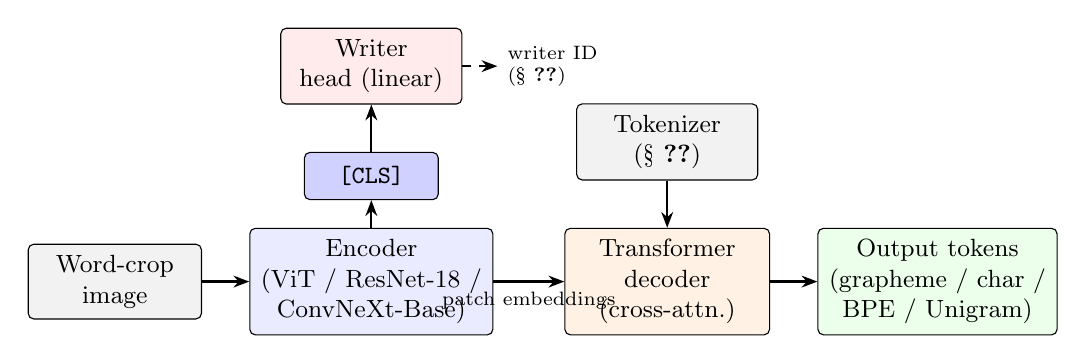
\begin{tikzpicture}[
  font=\small,
  box/.style={draw, rounded corners=2pt, align=center, minimum height=0.9cm, inner sep=4pt},
  enc/.style={box, fill=blue!8, minimum width=2.6cm},
  dec/.style={box, fill=orange!10, minimum width=2.6cm},
  head/.style={box, fill=red!8, minimum width=2.3cm},
  tok/.style={box, fill=green!8, minimum width=2.3cm},
  arr/.style={-{Stealth[length=2mm]}, thick}
]
  \node[box, fill=gray!10, minimum width=2.2cm] (img) {Word-crop\\ image};
  \node[enc, right=0.6cm of img] (enc) {Encoder\\ (ViT / ResNet-18 /\\ ConvNeXt-Base)};
  \node[box, fill=blue!18, above=0.35cm of enc, minimum width=1.7cm, minimum height=0.6cm] (cls) {\texttt{[CLS]}};
  \node[head, above=0.6cm of cls] (whead) {Writer\\ head (linear)};
  \node[dec, right=0.9cm of enc] (dec) {Transformer\\ decoder\\ (cross-attn.)};
  \node[tok, right=0.6cm of dec] (out) {Output tokens\\ (grapheme / char /\\ BPE / Unigram)};
  \node[box, fill=gray!10, above=0.6cm of dec, minimum width=2.3cm] (tokenizer) {Tokenizer\\ (\S~\ref{sec:tokenizers})};

  \draw[arr] (img) -- (enc);
  \draw[arr] (enc) -- (dec) node[midway, below, font=\scriptsize] {patch embeddings};
  \draw[arr] (enc) -- (cls);
  \draw[arr] (cls) -- (whead);
  \draw[arr] (dec) -- (out);
  \draw[arr] (tokenizer) -- (dec);
  \draw[arr, dashed] (whead) -- ++(1.6,0) node[right, font=\scriptsize, align=left] {writer ID\\ (\S~\ref{sec:unlearn-pipeline})};
\end{tikzpicture}
\caption{PATHOK's shared encoder-decoder pipeline. The tokenizer ablation
(\S~\ref{sec:tokenizers}) changes only the decoder's target vocabulary; the
writer-identification head (\S~\ref{sec:unlearn-pipeline}) is a linear
probe on the encoder's \texttt{[CLS]} embedding, trained jointly with
recognition but architecturally independent of it -- the two axes this
paper studies attach to the same frozen backbone at these two distinct
points.}
\label{fig:pipeline}
\end{figure}

\subsection{Tokenization Strategies}
\label{sec:tokenizers}

Three tokenizers are compared under an identical encoder and, where
recoverable across the project's separate per-tokenizer training runs,
an identical training protocol (Table~\ref{tab:hparams}):

\begin{itemize}
\item \textbf{Grapheme.} Splits text into extended grapheme clusters
  (Unicode UAX \#29 / \citealt{alam2021graphemes}), so a consonant
  conjunct such as \textit{ক্রা} remains a single token instead of
  fragmenting into its constituent codepoints.
\item \textbf{Character.} Splits into individual Unicode codepoints; each
  retains a consistent visual identity independent of surrounding context.
\item \textbf{Byte-Pair Encoding (BPE).} A subword vocabulary learned by
  greedy pairwise merging on the training corpus, following
  \citet{basher2023bngraphemizer}'s and \citet{hasan2025gradet}'s
  comparison baselines.
\end{itemize}

\subsection{Datasets and Experimental Protocol}
\label{sec:data}

The tokenizer and encoder ablations (Section~\ref{sec:agg-results}) train
and evaluate on BnHTRD \citep{rahman2023bnhtrd}, a document-level offline
Bangla handwritten text recognition benchmark with word-level bounding-box
annotations across 125 distinct writers. Word crops are extracted from
the annotated pages, filtered for legibility and non-empty ground truth,
and split 80/10/10 into train/validation/test at a fixed random seed
(seed~42) for the base recognition experiments (Sections
\ref{sec:agg-results}--\ref{sec:complexity}), giving the $n=6{,}614$-word
test set used throughout the sample-level divergence analysis. This split
is \emph{not} writer-disjoint -- a word from a given writer's page can
appear in both train and test -- which is standard practice for a pure
recognition benchmark but is deliberately replaced by a writer-disjoint
split for every writer-identity experiment in
Sections~\ref{sec:unlearn-pipeline} onward, for the reasons given there.

Section~\ref{sec:cross-dataset}'s cross-dataset generalization check
additionally evaluates the BnHTRD-trained TrOCR~+~grapheme checkpoint,
zero-shot and without any fine-tuning, on IIIT-Indic-HW-Words
\citep{gongidi2021iiitindic}, a separate Indic-script handwritten-word
dataset collected under a different acquisition pipeline, writer
population, and (for the non-Bangla portions of that dataset) script; only
its Bangla-script subset ($n=17{,}574$ words) is used here, so that
cross-dataset generalization is being measured independent of a
cross-script confound.

\begin{table}[h]
\caption{Training and decoding hyperparameters, all three tokenizer arms.
Shared rows apply identically across arms; the Character row's training
hyperparameters could not be recovered from the arm's surviving evaluation
script (data loading and split were confirmed identical; the training
notebook itself was not preserved) and are marked accordingly.}
\label{tab:hparams}
\begin{tabular*}{\tblwidth}{@{}LLLL@{}}
\toprule
 & Grapheme & BPE & Character \\
\midrule
Base model & \multicolumn{3}{l}{\texttt{microsoft/trocr-base-handwritten}} \\
Split (train/val/test) & \multicolumn{3}{l}{80/10/10, seed 42} \\
Max sequence length & \multicolumn{3}{l}{64 tokens} \\
Vocab size & data-derived & 2{,}000 (SentencePiece BPE) & data-derived \\
Batch size (train/eval) & 16 / 16 & 16 / 16 & \textit{not recovered} \\
Epochs (cap, early stop) & 5, patience 3 & 5, patience 4 & \textit{not recovered} \\
Learning rate & 5e-5 & 5e-5 & \textit{not recovered} \\
Weight decay & 0.01 & 0.01 & \textit{not recovered} \\
Decoding & beam, $k{=}4$ & beam, $k{=}4$ & \textbf{beam, $k{=}2$} \\
\bottomrule
\end{tabular*}
\end{table}

The decoding mismatch in the table's last row -- Character was evaluated
with half the beam width of the other two arms -- was only caught during a
methodology audit after the fact. \todo{Re-decode the Character test set at
$k{=}4$ for a directly comparable number before submission; on
current evidence a doubled beam width is very unlikely to close a
92.21\%-vs-88.54\% word-accuracy gap of this size, but the exact
Character CER/WER figures in
Tables~\ref{tab:tokenizer-ablation}--\ref{tab:contingency} should be
treated as a slightly pessimistic lower bound until that re-run is done.}

\subsection{Sample-Level Divergence Methodology}
\label{sec:divergence-method}

Beyond aggregate CER/WER, per-sample predictions from the three tokenizer
checkpoints were merged on the identical BnHTRD test set
($n=6{,}614$). For each sample the outcome is labeled by which of the three
models produced the correct word, giving a $2^3$ contingency table (Table
\ref{tab:contingency}). Statistical significance between any pair of
tokenizers is assessed with McNemar's exact test on the discordant pairs
(cases where exactly one of the two models is correct), which is the
appropriate paired test for two classifiers scored on the same items.

Each ground-truth word is additionally annotated with complexity features
computed via the same extended-grapheme-cluster segmentation used by the
grapheme tokenizer itself: grapheme count, presence of $\geq 1$ consonant
conjunct (a grapheme containing a \textit{hasanta}, U+09CD), and the ratio
of character length to grapheme length (a proxy for how much a
codepoint-level tokenizer must ``reassemble'' relative to the visual unit
count).

\subsection{Writer-Identity Architecture and Unlearning Pipeline}
\label{sec:unlearn-pipeline}

The best recognition configuration (TrOCR + grapheme tokenization) is
extended with a linear writer-classification head on the encoder's CLS
token, trained jointly with the recognition objective. BnHTRD's 125
writers are partitioned into a writer-disjoint split -- 74 retain writers
(38{,}275 words), 20 forget writers (7{,}739 words), and 30 held-out test
writers (18{,}067 words, used only as MIA non-members) -- frozen once and
reused across every experiment reported in Section~\ref{sec:unlearn-results}.
A random, non-writer-disjoint split (as used by the base recognition
system) is unsuitable here: it would let writer identity leak into
``unseen'' evaluation samples and would leave no valid non-member class for
membership inference.

\begin{figure}[h]
\centering
\begin{tikzpicture}[font=\small]
  \def\totalw{125}
  \def\retw{74} \def\forw{20} \def\tesw{30}
  \def\barw{7.2cm} \def\barh{0.55cm}
  \pgfmathsetmacro{\retwidth}{\barw*\retw/\totalw}
  \pgfmathsetmacro{\forwidth}{\barw*\forw/\totalw}
  \pgfmathsetmacro{\teswidth}{\barw*\tesw/\totalw}
  \pgfmathsetmacro{\forx}{\retwidth}
  \pgfmathsetmacro{\tesx}{\retwidth+\forwidth}
  \draw[fill=blue!15, draw=blue!50!black] (0,0) rectangle (\retwidth,\barh)
    node[midway, font=\scriptsize] {Retain (74w)};
  \draw[fill=red!15, draw=red!60!black] (\forx,0) rectangle (\tesx,\barh)
    node[midway, font=\scriptsize] {Forget};
  \draw[fill=gray!15, draw=gray!60!black] (\tesx,0) rectangle (\barw,\barh)
    node[midway, font=\scriptsize] {Test};
  \node[below=2pt] at (\retwidth/2, 0) {\tiny \textbf{38{,}275 words}, classifier member, seen in training};
  \node[below=2pt, align=center] at ({(\forx+\tesx)/2}, -0.42) {\tiny \textbf{7{,}739 words} (20w)\\ \tiny member, unlearning target};
  \node[below=2pt, align=center] at ({(\tesx+\barw)/2}, -0.42) {\tiny \textbf{18{,}067 words} (30w)\\ \tiny non-member, MIA only};
\end{tikzpicture}
\caption{BnHTRD writer-disjoint split, drawn to scale by writer count
(125 total, per the frozen split's own record -- see the open question
below on whether retain is 74 or 75 of them). Only retain and forget
writers are ever classes of the writer head; test writers are held out
entirely, used only as the non-member class for membership inference
(Section~\ref{sec:audit}).}
\label{fig:split}
\end{figure}

\openq{An internal split-integrity check script preserved from this
study's Kaggle pipeline records the frozen split as \texttt{writers:\ 125},
\texttt{classes:\ 95} (i.e.\ retain writers $+$ forget writers $=95$),
which -- at forget $=20$ -- implies 75 retain writers, not the 74 reported
in the surviving thesis text and reproduced here. The word counts
(38{,}275 / 7{,}739 / 18{,}067) match exactly either way, so this is a
one-writer bookkeeping discrepancy rather than a data-leakage or
sample-count error, and it does not move any accuracy, CER, or
significance-test number in this paper (all of which are computed
directly from the frozen split's word-level files, not from the writer
count). It should still be resolved against the original \texttt{split.json}
before submission, since Figure~\ref{fig:split} and every ``$74$ retain
writers'' / ``chance $\approx 1.35\%$ over 74 classes'' statement in this
paper (Sections~\ref{sec:unlearn-pipeline},~\ref{sec:arf-results}) would
shift by one writer -- e.g.\ chance for a 75-writer denominator is
1.33\%, not 1.35\% -- if 75 is the correct figure.}

\textbf{Stage~I (pruning).} Following \citet{kang2026privacy}, encoder
feed-forward units are ranked by an importance score
$(\mathrm{act}_{\text{forget}}+\epsilon)/(\mathrm{act}_{\text{retain}}+\epsilon)$
computed from mean absolute activations on forget- vs.\ retain-writer
batches, and the top-ranked units per depth group (shallow/middle/deep) are
zeroed.

\textbf{Stage~II (unlearning objectives).} Five objectives from
\citet{kang2026privacy} are implemented on top of the pruned checkpoint:
Writer-ID Confusion (WIC, KL divergence of the writer head's output to a
uniform distribution on forget batches), Random Labeling (forget-writer
labels permuted onto retain-writer classes), Fisher Forgetting (a single
diagonal-Fisher-scaled gradient step, $\theta \leftarrow \theta - \alpha\,
g_f/(F+\mu)$), Amnesiac Unlearning (gradient ascent on the forget-writer
classification loss), and DELETE (masked knowledge distillation against a
frozen teacher, with forget-class logits set to $-\infty$ in both teacher
and student before the softmax).

\subsection{Privacy Audit Instruments}
\label{sec:audit}

Three independent instruments audit each unlearned checkpoint:

\begin{enumerate}
\item \textbf{Membership-inference (MIA) gate.} A 12-dimensional
  teacher-forced recognition-confidence feature vector (mean/min/max/std
  log-probability, entropy, margin, rank statistics) feeds a logistic
  regression classifier trained on retain (member) vs.\ test (non-member)
  samples, then applied to the forget set.
\item \textbf{Few-shot frozen-encoder probe.} A linear classifier is
  trained \emph{from scratch, after unlearning, on the frozen encoder} to
  identify forget writers from $k \in \{1,2,3,5,\ldots,150\}$ support
  examples per writer, and compared against an identical probe on
  genuinely unseen (test-split) writers. This measures whether writer
  identity survives in the representation independent of the
  classification head.
\item \textbf{Relearning attack.} An attacker is given $k \in \{1,2,3,5\}$
  real words per forgotten writer and $\leq 150$ fine-tuning steps,
  \emph{with retain-set replay interleaved at every step} so that recovery
  cannot be explained by the attack silently retraining the whole model.
  Retain-set accuracy is tracked throughout as a validity gate.
\end{enumerate}

\subsection{Representation-Level Forgetting: ARF and MGDA}
\label{sec:arf-mgda}

Two further methods test whether attacking the representation directly, in
the spirit of \citet{wang2026rfuss}, improves on output-level suppression
-- without retrofitting their Variational Information Bottleneck
architecture onto a model whose CLS embedding is deterministic, not a
stochastic latent, and for which no $I(Z;X)$ estimator is defined.

\textbf{Adversarial Representation Forgetting (ARF).} A freshly initialized
probe is trained to identify forget writers directly from the ViT CLS
embedding $z$; a gradient-reversal layer \citep{ganin2015dann} between $z$
and the probe pushes the encoder to defeat it, with the probe periodically
reinitialized (every 100 steps) so the encoder cannot simply learn to fool
one fixed adversary the way it can fool WIC's static uniform-distribution
target. The model's own writer head is additionally suppressed via the WIC
mechanism, purely so output-level metrics remain comparable across all
eight methods; the representation-level test is the independent post-hoc
probe of Section~\ref{sec:audit}, which never observes ARF's internal
training-time adversary.

\textbf{MGDA-weighted objectives.} \citeauthor{wang2026rfuss}'s
parameter-self-sharing contribution -- a closed-form, per-step
Pareto-stationary blend weight $\hat\alpha_u$ between a forgetting-objective
gradient $g_u$ and a remembering-objective gradient $g_r$ on shared
parameters \citep{sener2018mtl,desideri2012mgda} -- is architecture-agnostic
and is applied as a drop-in replacement for the fixed loss weights in WIC
and Random Labeling:
\begin{equation}
\hat\alpha_u = \left[\, \frac{(g_r-g_u)^{\!\top} g_r}{\lVert g_r-g_u \rVert_2^2} \,\right]_{+,\,1},
\qquad
g_{\text{final}} = \hat\alpha_u\, g_u + (1-\hat\alpha_u)\, g_r,
\label{eq:mgda}
\end{equation}
where $[\cdot]_{+,1}$ clips to $[0,1]$. This is tested as a separate
experiment from ARF, isolating whether dynamic weighting alone -- with no
representation-level attack -- improves on fixed-weight output suppression.

%% ====================================================================
\section{Results}
\label{sec:results}
%% ====================================================================

\subsection{Aggregate Recognition Results}
\label{sec:agg-results}

\begin{table}[h]
\caption{Encoder ablation, grapheme tokenization held constant. The
ConvNeXt-Base row is a later addition (Section~\ref{sec:apples-to-apples}),
run under the identical protocol as the two rows above it; its throughput
was not measured on the same basis as the other two and is omitted rather
than implying a comparison that was not actually made.}
\label{tab:encoder-ablation}
\begin{tabular*}{\tblwidth}{@{}LLLLL@{}}
\toprule
Encoder & Params & Word Acc.\ (\%) & CER (\%) & Throughput (samp./s) \\
\midrule
ResNet-18 CNN & 37.4M & 83.88 & 8.36 & $\approx$27 \\
TrOCR ViT & $\sim$334M & \textbf{92.21} & \textbf{2.52} & $\approx$3.5 \\
ConvNeXt-Base & $\sim$372M & 91.70 & 2.63 & -- \\
\bottomrule
\end{tabular*}
\end{table}

\subsection{A genuine apples-to-apples encoder comparison, and two robustness checks on the headline number}
\label{sec:apples-to-apples}

Section~\ref{sec:arf-results} reports ConvNeXt-Base's recognition
performance too, but under the writer-disjoint split and joint
recognition-plus-writer-identification recipe that section's investigation
required, decoded greedily rather than with beam search -- a real but
looser comparison (7.58\% vs.\ the ViT oracle's 7.74\% CER) across two
protocol differences at once. The ConvNeXt-Base row added to
Table~\ref{tab:encoder-ablation} closes that gap: same standard 80/10/10
split as the ResNet-18 and ViT rows above it, same grapheme tokenizer and
vocabulary code, same fixed hyperparameters (learning rate $5\times
10^{-5}$, 500 warmup steps, weight decay 0.01, batch size 16, up to 5
epochs with early-stopping patience 3), same beam-4 test-set decoding. No
writer-identification head this time -- recognition only, isolating
architecture from every other variable. Under this genuinely controlled
comparison, ConvNeXt-Base lands within half a point of ViT on word
accuracy (91.70\% vs.\ 92.21\%) and about a tenth of a point on CER
(2.63\% vs.\ 2.52\%) -- a tighter match than the looser comparison above,
and the strongest evidence in this paper that the recognition side of the
architecture-family question is close to a genuine tie, even as
Section~\ref{sec:arf-results} shows the writer-identification side is not.

\textbf{Is ResNet-18's gap a decoder-capacity artifact?} Table~\ref{tab:encoder-ablation}
pairs ResNet-18's 11.2M-parameter CNN encoder with the same lightweight
custom \texttt{nn.TransformerDecoder} throughout this paper (26.2M
parameters, $d_{\text{model}}{=}512$), while both ViT and ConvNeXt-Base
carry TrOCR's pretrained 196.8M-parameter decoder -- an order-of-magnitude
difference that leaves open whether ResNet-18's 8-point recognition
deficit is really an encoder-quality effect or simply reflects its
much smaller decoder. To isolate this, ResNet-18's decoder was scaled up
to the same architectural \emph{style} ($\mathrm{dim}_{\text{ff}}{=}4
d_{\text{model}}$, 6 layers, dropout 0.1) at $d_{\text{model}}{=}1424$,
$\mathrm{nhead}{=}16$ -- a closed-form parameter count, verified exactly
against a live PyTorch instantiation before training, of 197.7M, matching
ConvNeXt's decoder to within 0.5\%. Trained from scratch under the same
protocol as the original ResNet-18 arm (10 epochs, Adam $10^{-4}$,
\texttt{ReduceLROnPlateau}, batch 32, identical 80/10/10 split), the
scaled-decoder variant reached 81.24\% word accuracy, 16.54\% CER, and
18.76\% WER -- \emph{worse} than the original 26.2M-parameter decoder
(83.88\%, 8.36\%, 16.12\%) on every metric, not better. Training was also
visibly less stable: validation CER oscillated between 13.86\% and
46.59\% across epochs 6--8 with a fixed learning rate and no warmup,
where the small-decoder arm converged smoothly. Matching the decoder
parameter count of ViT and ConvNeXt-Base does not close any of ResNet-18's
gap to them; if anything, the larger decoder is harder to optimize on top
of an unchanged 11.2M-parameter encoder without a matching increase in
encoder capacity or a warmup schedule tuned for it. This is consistent
with the gap being substantially an \emph{encoder}-capacity effect (11.2M
parameters vs.\ ViT's 86.7M or ConvNeXt's 88.4M) rather than a decoder
one, though it does not rule out that a better-tuned optimizer schedule
for the larger decoder specifically might recover some of the loss.

Two further checks target the headline TrOCR~+~grapheme number itself
rather than the architecture comparison. First, \texttt{encode\_label()}
in the recognition pipeline prepends an explicit beginning-of-sequence
token to every label, but \texttt{VisionEncoderDecoderModel} \emph{also}
prepends \texttt{decoder\_start\_token\_id} (the same token) via
\texttt{shift\_tokens\_right()} whenever no explicit
\texttt{decoder\_input\_ids} is supplied -- which this pipeline never
does. The practical effect is that every model in this paper was trained
with a doubled beginning-of-sequence token at the start of its decoder
input, a token \texttt{generate()} never actually supplies at inference
(a single beginning-of-sequence token only). Retraining ConvNeXt-Base with
this corrected -- single beginning-of-sequence -- label encoding, holding
everything else in Table~\ref{tab:encoder-ablation}'s protocol fixed,
produced a very slightly \emph{worse} result (91.41\% word accuracy,
2.84\% CER) than the faithful reproduction of the original encoding
reported above, not a better one. The direction is opposite to what a
train/inference mismatch account would naively predict, though the gap
(0.3 points) is well within the range a single run's noise could produce;
we read this as evidence the doubled-token artifact is not costing this
architecture-family comparison anything measurable, rather than as
confirmation it never matters anywhere. \openq{Whether this null result
holds on the ViT encoder itself -- rather than only on ConvNeXt, tested
here as a byproduct of the encoder comparison -- is being tested directly
as this manuscript is being prepared and is not yet resolved; the
mechanism (Section~\ref{sec:limitations}) predicts the doubled token
should be harmless precisely because it is a consistent artifact of every
training example, which a sufficiently expressive decoder can learn to
absorb by simply emitting it as a free first generation step -- a
prediction that should hold across encoders if it holds at all, but has
only been tested on one so far.}

Second, a coarse hyperparameter sweep (10 configurations: five learning
rates $\times$ two warmup ratios, screened on an 8{,}000-image subsample
before the winning configuration was retrained at full scale) found a
configuration -- the original learning rate with a $3\times$ larger warmup
ratio -- that outperformed the headline setup by a wide margin on the
short screen (12.67\% vs.\ 17.71\% validation CER at matched, deliberately
limited step count). That advantage did not survive scaling to the full
5-epoch training budget: the tuned configuration's test-set result
(92.21\% word accuracy, 2.50\% CER) is statistically indistinguishable
from the original, untuned headline number (92.21\%, 2.52\%). Read
together with the recognition side of Table~\ref{tab:encoder-ablation},
this is consistent with the headline $\sim$2.5\% CER sitting closer to a
capacity or data ceiling for this encoder-decoder pair than an
optimization one: substantially different learning-rate/warmup schedules
converge to the same place given enough epochs, and a different encoder
family (ConvNeXt-Base) reaches nearly the same place too.

\begin{table}[h]
\caption{Tokenizer ablation, TrOCR ViT encoder held constant.}
\label{tab:tokenizer-ablation}
\begin{tabular*}{\tblwidth}{@{}LLLL@{}}
\toprule
Tokenizer & Word Acc.\ (\%) & CER (\%) & WER (\%) \\
\midrule
Grapheme & \textbf{92.21} & \textbf{2.52} & \textbf{7.79} \\
BPE, vocab 500 & 91.02 & 3.11 & 8.98 \\
Character & 88.54 & 3.30 & 11.46 \\
SentencePiece Unigram, vocab 500 & 89.02 & 3.76 & 10.98 \\
SentencePiece Unigram, vocab 2000 & 89.34 & 3.99 & 10.66 \\
WordPiece, vocab 2000 & 88.81 & 4.10 & 11.19 \\
BPE, vocab 2000 & 87.77 & 4.25 & 12.23 \\
BPE, vocab 4000 & 86.15 & 5.59 & 13.85 \\
\bottomrule
\end{tabular*}
\end{table}

\begin{figure}[h]
\centering
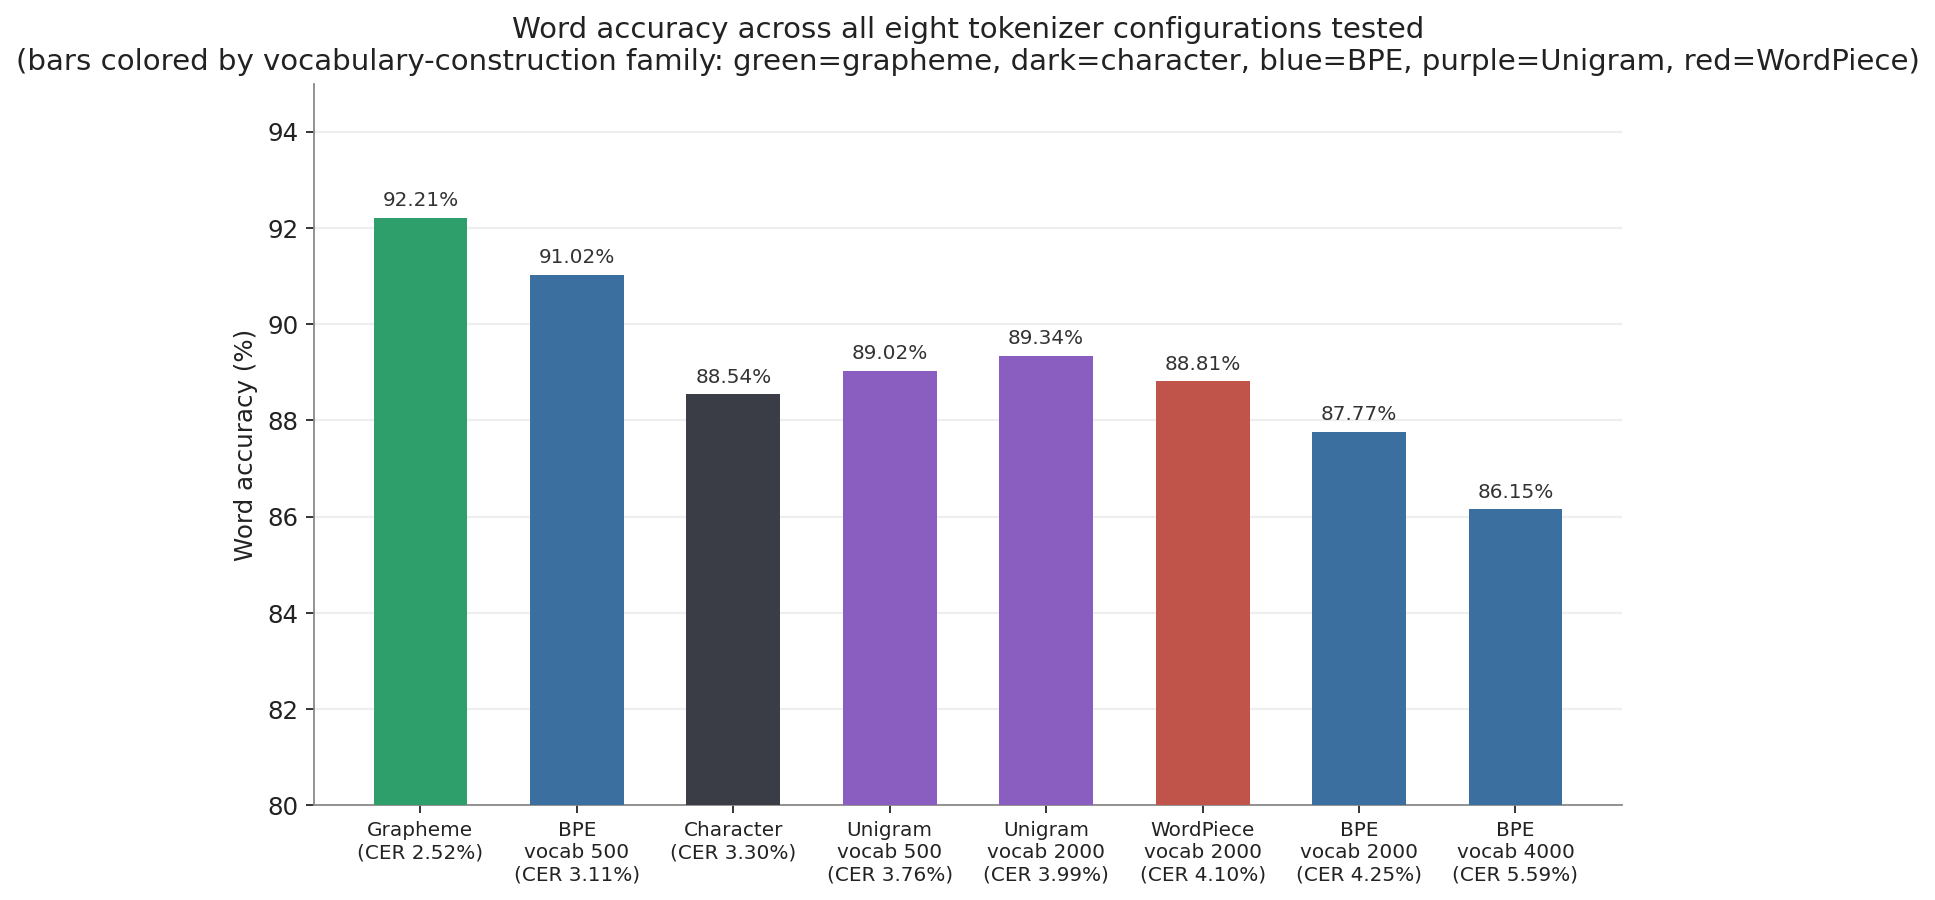
\includegraphics[width=\linewidth]{figs/fig_tokenizer_sweep.png}
\caption{Word accuracy across all eight tokenizer configurations tested
(Table~\ref{tab:tokenizer-ablation}), colored by vocabulary-construction
family. Vocabulary size (BPE 500 vs.\ 2000 vs.\ 4000) moves accuracy more
than the choice of merge algorithm at fixed size (BPE~2000 vs.\ WordPiece
2000 vs.\ Unigram 2000, which rank in exactly that order); Unigram's own
accuracy is comparatively flat across the same 500-to-2000 vocabulary
range (89.02\% vs.\ 89.34\%) where BPE swings by over three points, an
asymmetry discussed below.}
\label{fig:tokenizer-sweep}
\end{figure}

The original three-way ablation was independently re-derived this study
from per-sample prediction logs of all three trained checkpoints and
matched their originally reported aggregates exactly. Two further
tokenizer variants (Experiment 4) extend it under an identical protocol
(row-level split, matching the original three-way comparison rather than
the writer-disjoint split used elsewhere in this paper; see
Section~\ref{sec:limitations}), changing exactly one factor each from the
BPE arm above.

\textbf{Vocabulary size.} Sweeping BPE's vocabulary size while holding
everything else constant produces a clean, monotonic result in the
opposite direction from what a larger, more expressive vocabulary might
suggest: 500 (91.02\% word accuracy) outperforms 2{,}000 (87.77\%), which
outperforms 4{,}000 (86.15\%). Smaller BPE vocabularies perform
\emph{better} on this task, not worse -- consistent with a
visual-instability account (Section~\ref{sec:discussion}): a larger
subword vocabulary means more distinct merge tokens compete for
increasingly rare training signal, and each one is a longer, more
compound handwritten shape for the same greedy-merge instability to act
on. At vocab 500, BPE (91.02\%) closes most of the gap to grapheme
(92.21\%) and edges past character tokenization (88.54\%) -- vocabulary
size, not the merge algorithm alone, accounts for a substantial share of
BPE's original deficit against the other two tokenizers.

\textbf{Merge algorithm.} Holding vocabulary size fixed at 2{,}000 and
replacing BPE's greedy pairwise merging with SentencePiece's Unigram
language-model tokenization improves word accuracy from 87.77\% to
89.34\% and CER from 4.25\% to 3.99\% -- a real improvement, consistent
with reports that Unigram outperforms BPE in other low-resource settings,
but a smaller effect than the vocabulary-size sweep above and still short
of both grapheme and the vocab-500 BPE arm. The two factors are not
redundant: switching algorithms at fixed vocabulary size and shrinking
vocabulary at a fixed algorithm each move word accuracy by 1.6--3.3
points independently, so BPE's original deficit against grapheme
tokenization reflects a combination of both factors rather than either one
alone.

\textbf{A third merge algorithm, same fixed vocabulary.} WordPiece
(BERT's algorithm) sits on the same vocab-2{,}000 axis as the BPE/Unigram
comparison above, changing only the merge-scoring criterion: BPE picks
each merge by raw pair frequency, Unigram prunes a large seed vocabulary
by language-model likelihood, and WordPiece picks each merge by the
likelihood \emph{improvement} a pair contributes ($\mathrm{freq(pair)} /
(\mathrm{freq(a)} \cdot \mathrm{freq(b)})$) -- a greedy procedure like
BPE's, but scored by something closer to Unigram's probabilistic
criterion. Trained and evaluated under the identical protocol, WordPiece
reaches 88.81\% word accuracy (4.10\% CER, 11.19\% WER) -- landing
between BPE (87.77\%) and Unigram (89.34\%) at the same vocabulary size,
in exactly the order its algorithm's position between the two would
predict. This is a single data point, not a swept curve, but the clean
ordering (BPE $<$ WordPiece $<$ Unigram, tracking how much of a
language-model criterion each algorithm's merge step actually uses) is
consistent with the vocabulary-economy account of grapheme's advantage
discussed below: the more a subword algorithm's merge criterion
resembles a stability-seeking probabilistic objective rather than raw
frequency, the closer it gets to grapheme's fixed, collision-free
vocabulary -- without fully reaching it.

\textbf{Unigram's vocabulary-size sensitivity, filled in at 500.} Running
Unigram at vocab 500 under the same protocol -- completing the
$2\times2$ algorithm-by-vocabulary-size grid for the one BPE vocabulary
size it had been missing -- gives 89.02\% word accuracy (3.76\% CER,
10.98\% WER), a hair \emph{below} Unigram's own vocab-2000 result
(89.34\%, 3.99\% CER) rather than above it. This is the opposite pattern
from BPE, where shrinking the vocabulary from 2{,}000 to 500 was worth
3.25 points (87.77\% $\rightarrow$ 91.02\%): Unigram's accuracy is
essentially flat across the same range (89.34\% $\rightarrow$ 89.02\%, a
0.32-point difference well within what a single training run's noise
could produce). Unigram's language-model-based tokenization already
tends toward a more stable, lower-collision vocabulary than BPE's greedy
pairwise merges even at a larger nominal size, which is consistent with
shrinking the vocabulary buying BPE most of the way to Unigram's
stability while leaving Unigram itself with little left to gain from the
same shrink -- though with one run per configuration this reads as a
plausible reading of the pattern, not a claim the two algorithms respond
differently to vocabulary size with statistical confidence.

\openq{Table~\ref{tab:tokenizer-ablation} does not yet disentangle two
candidate mechanisms for grapheme tokenization's remaining edge over even
the best-tuned BPE variant (92.21\% vs.\ vocab-500 BPE's 91.02\%): (i) a
\emph{linguistic-alignment} account, where grapheme clusters are the
mechanism because they are the actual visual unit a Bangla writer produces
stroke-by-stroke, so aligning tokens to them is specifically what helps;
or (ii) a \emph{vocabulary-economy} account, where what matters is simply
having a small, stable, low-collision target vocabulary, and grapheme
clustering is one way to get one, not the reason it works. The vocab-size
sweep is consistent with either: it shows vocabulary size matters a
great deal, but grapheme tokenization's own vocabulary size is
data-derived and was never itself swept. A clean test would train a
BPE-style vocabulary constrained to merge only within grapheme-cluster
boundaries (isolating cluster-alignment from vocabulary size and merge
algorithm, both of which Table~\ref{tab:tokenizer-ablation} already
varies independently) -- not run in this study.}

\subsection{Sample-Level Significance}
\label{sec:sample-sig}

\begin{table}[h]
\caption{Full 3-way outcome distribution on the BnHTRD test set
($n=6{,}614$). G/B/C = correct under Grapheme/BPE/Character tokenization.}
\label{tab:contingency}
\begin{tabular*}{\tblwidth}{@{}LLLL@{}}
\toprule
Outcome & $n$ & Outcome & $n$ \\
\midrule
GBC (all correct) & 5{,}293 & C only & 100 \\
GC & 369 & BC & 94 \\
GB & 333 & B only & 85 \\
\textbf{G only} & \textbf{104} & None correct & 236 \\
\bottomrule
\end{tabular*}
\end{table}

McNemar's exact test, paired on the same 6{,}614 items: Grapheme vs.\ BPE
(473 grapheme-only-correct vs.\ 179 BPE-only-correct, $p=1.6\times
10^{-31}$); Grapheme vs.\ Character (437 vs.\ 194, $p=1.7\times 10^{-22}$).
The aggregate CER gap of Section~\ref{sec:agg-results} is not a
corpus-level artifact but an overwhelming sample-level effect against both
baselines independently. 104 words (1.6\% of the test set) are
\emph{triple-divergence} cases: grapheme tokenization correct while
\emph{both} baselines are wrong on the same word.

\subsection{Complexity-Conditioned Analysis}
\label{sec:complexity}

\begin{figure}[h]
\centering
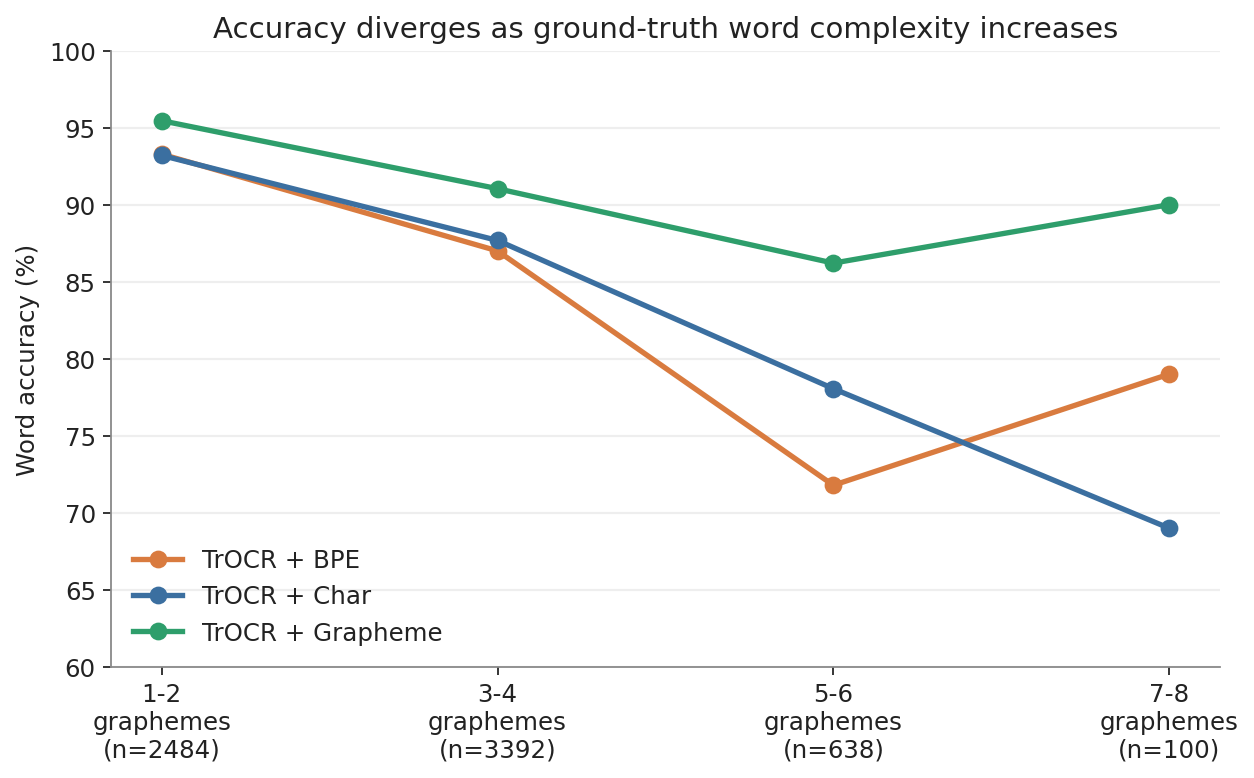
\includegraphics[width=\linewidth]{figs/fig_outcome_by_gcount.png}
\caption{Word accuracy for all three tokenizers vs.\ ground-truth grapheme
count. Character tokenization's advantage over BPE inverts at 7--8
graphemes (69\% vs.\ 79\%); grapheme tokenization does not collapse at
this length (90\%).}
\label{fig:by-gcount}
\end{figure}

\begin{figure}[h]
\centering
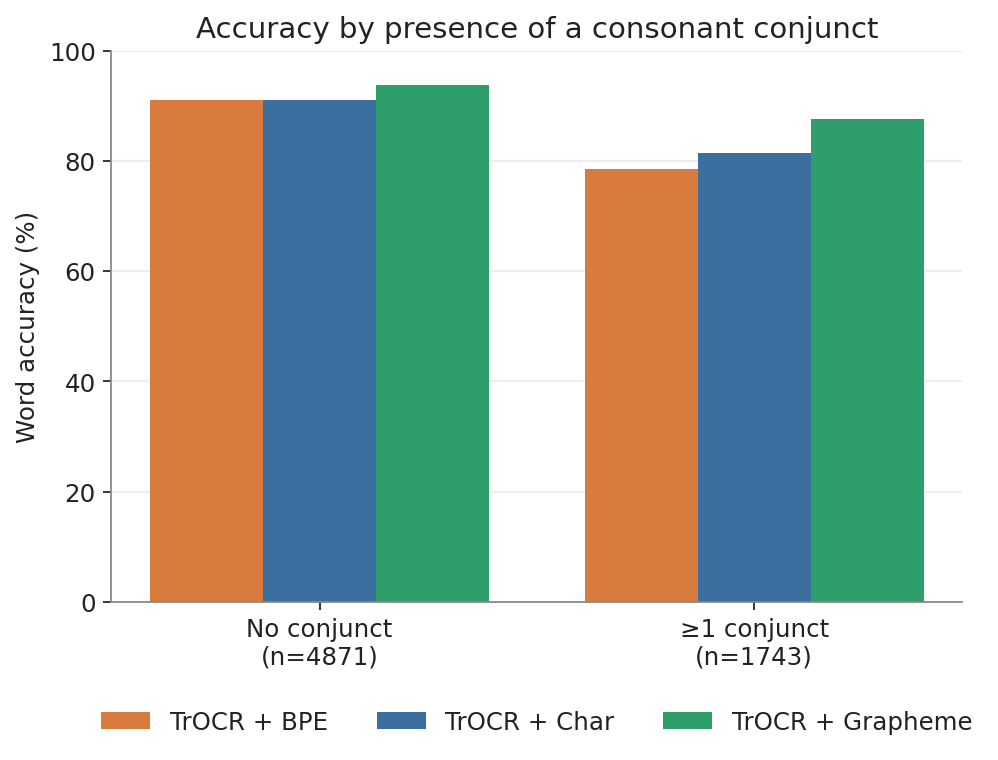
\includegraphics[width=\linewidth]{figs/fig_outcome_by_conjunct.png}
\caption{Word accuracy for all three tokenizers, grouped by presence of a
consonant conjunct in the ground-truth word.}
\label{fig:by-conjunct}
\end{figure}

With $\geq 1$ consonant conjunct present, accuracy on conjunct words is
87.6\% (grapheme), 81.5\% (character), 78.5\% (BPE), against 91--94\% for
all three on conjunct-free words -- grapheme's unique-win rate against BPE
more than doubles on conjunct words (5.3\%~$\to$~12.4\%). Bootstrapped 95\%
confidence intervals (5{,}000 resamples) confirm all three of these
differences hold up: [86.1, 89.1] vs.\ [79.6, 83.2] vs.\ [76.6, 80.4] for
conjunct words, non-overlapping across all three tokenizers.

Figure \ref{fig:by-gcount} shows character tokenization's point-estimate
advantage over BPE apparently inverting at the longest word-length bucket
(7--8 graphemes: 69.0\% character vs.\ 79.0\% BPE, against character
leading at every shorter bucket). We tested this formally with a logistic
regression of correctness on grapheme-cluster count, tokenizer identity,
and their interaction (pooled across all bucket boundaries rather than the
coarse 4-bin split, $n=13{,}228$ tokenizer-sample pairs): the
length$\times$tokenizer interaction is \emph{not} statistically
significant ($\beta=0.021$, $p=0.29$), and the 7--8 bucket itself has only
$n=100$ words with bootstrapped CIs for character [60.0, 78.0] and BPE
[71.0, 87.0] that overlap substantially. We therefore do not report this as
a confirmed crossover: it is a suggestive point-estimate reversal in an
underpowered tail bucket that a formal test does not support, and we flag
it as exactly the kind of small-sample pattern that should not be
overclaimed. The corresponding grapheme-vs-BPE interaction, by contrast,
\emph{is} significant and positive ($\beta=0.137$, $p=0.002$): grapheme's
advantage over BPE formally widens with word length, consistent with
longer words containing more conjuncts and reinforcing
Section~\ref{sec:sample-sig}'s conjunct-localization result rather than
complicating it.

\begin{figure}[h]
\centering
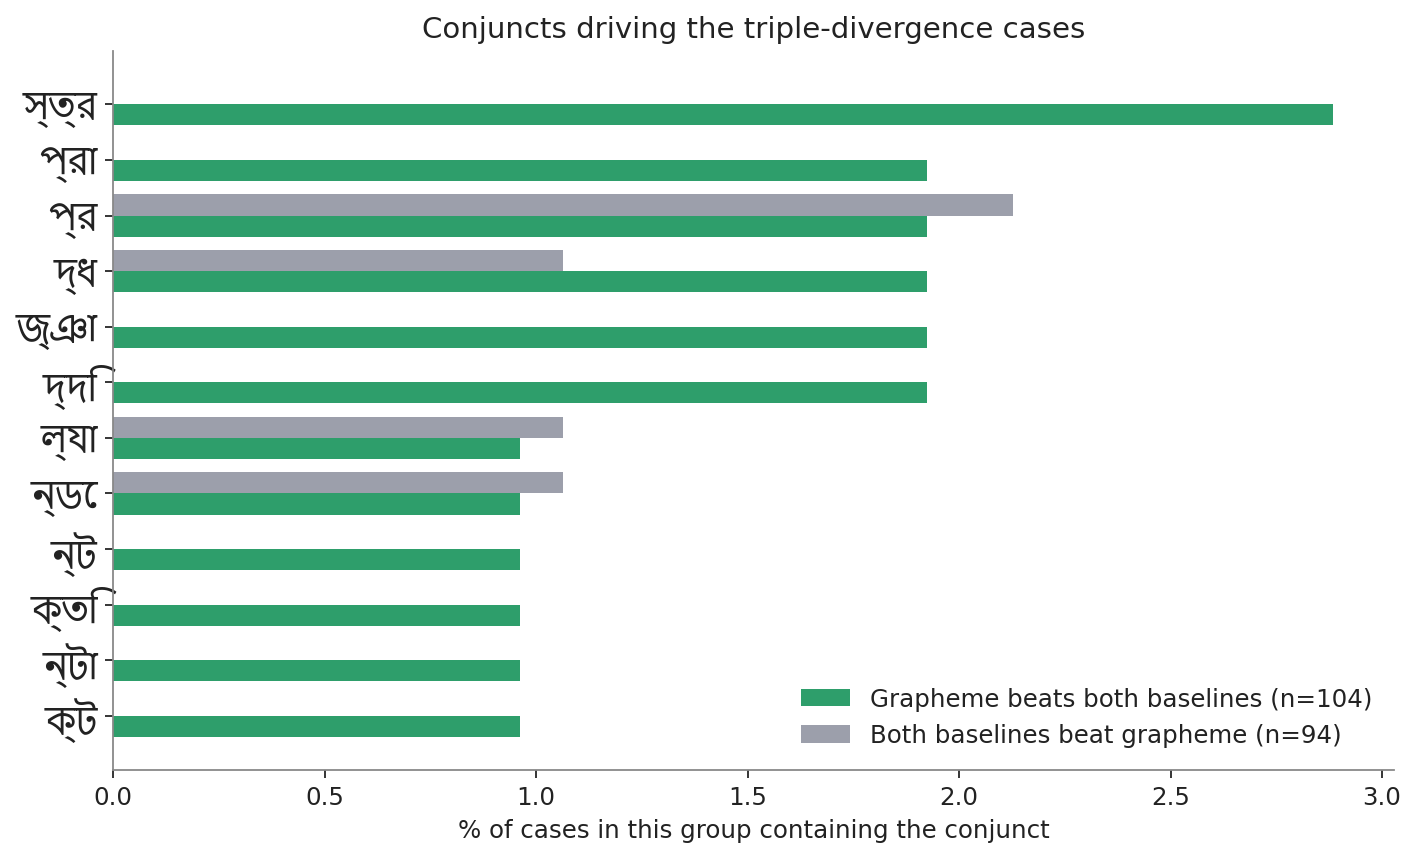
\includegraphics[width=\linewidth]{figs/fig_top_conjuncts.png}
\caption{Conjuncts most associated with the 104 grapheme-wins vs.\ 94
baselines-win triple-divergence cases.}
\label{fig:top-conjuncts}
\end{figure}

\subsection{Qualitative Evidence}
\label{sec:qualitative}

\begin{figure}[h]
\centering
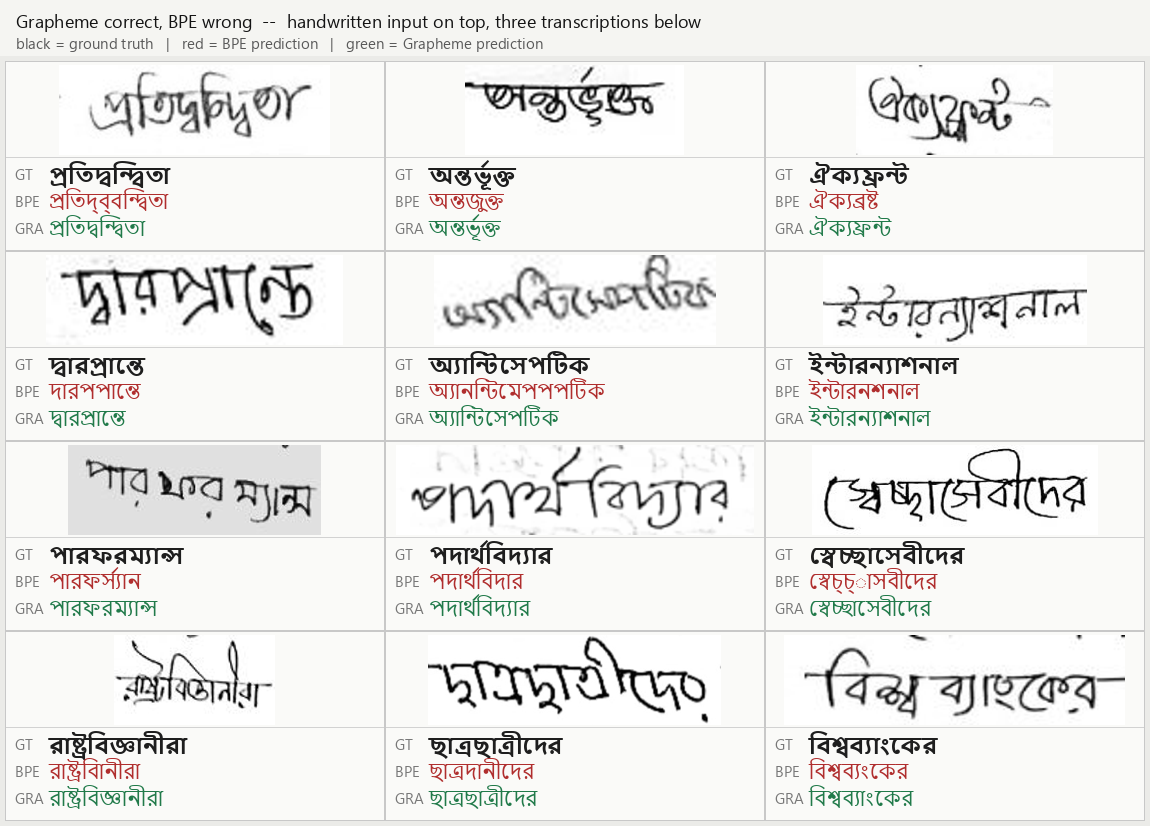
\includegraphics[width=\linewidth]{figs/fig_qualitative_grid.png}
\caption{Twelve handwriting samples where grapheme tokenization is correct
and BPE is wrong; predictions from both models shown beneath each image.}
\label{fig:qual-grid-bpe}
\end{figure}

\begin{figure}[h]
\centering
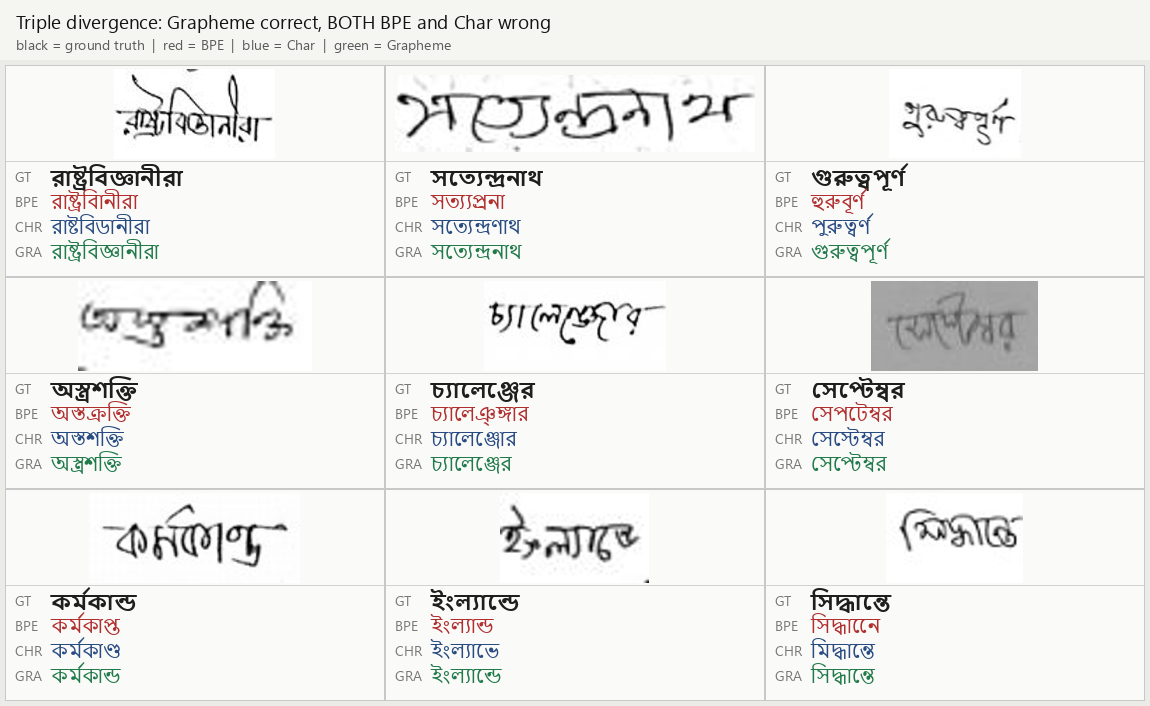
\includegraphics[width=\linewidth]{figs/fig_triple_divergence_grid.png}
\caption{Nine triple-divergence examples: grapheme tokenization correct
while both BPE and character tokenization are wrong on the same word.}
\label{fig:qual-grid-triple}
\end{figure}

\subsection{Cross-Dataset Generalization}
\label{sec:cross-dataset}

\begin{table}[h]
\caption{Zero-shot cross-dataset evaluation of TrOCR + Grapheme, trained
exclusively on BnHTRD.}
\label{tab:cross-dataset}
\begin{tabular*}{\tblwidth}{@{}LLLLL@{}}
\toprule
Eval.\ set & $n$ & Word Acc.\ (\%) & CER (\%) & WER (\%) \\
\midrule
BnHTRD (in-domain) & 6{,}614 & 92.21 & 2.52 & 7.79 \\
IIIT-Indic (out-of-domain) & 17{,}574 & 42.59 & 20.66 & 57.41 \\
\bottomrule
\end{tabular*}
\end{table}

The zero-shot gap between BnHTRD and IIIT-Indic (92.21\%~$\to$~42.59\%
word accuracy, 2.52\%~$\to$~20.66\% CER) is large but expected for a model
never fine-tuned on the target dataset: the two datasets differ in writer
population, vocabulary distribution, and image acquisition pipeline
(scanning/photography conditions, crop tightness, and background), any of
which alone can shift a recognition model trained on one benchmark. The
more informative number is not the aggregate gap but its shape:
catastrophic failures (predictions with CER $>50\%$, i.e.\ the model
producing an output nearly unrelated to the ground truth rather than a
plausible near-miss) stay comparatively rare on the out-of-domain set,
consistent with the model degrading gracefully rather than failing
qualitatively differently out-of-domain. \todo{The exact catastrophic-failure
rates (9.8\% out-of-domain vs.\ 0.9\% in-domain) are carried over from the
underlying thesis's Section 4.3.3 and were not independently re-derived
from IIIT-Indic per-sample logs this session; re-verify against a fresh
per-sample CER histogram on both sets before submission, and report the
CER threshold used to define ``catastrophic'' explicitly (a natural choice
is CER $>50\%$, but the thesis text does not confirm this was the
threshold actually used).} This graceful-degradation reading is also
consistent with Section~\ref{sec:arf-results}'s finding that recognition
capability itself transfers well across datasets and even across
scripts (ConvNeXt and ViT both reached comparable recognition performance
on BanglaWriting and on the English IBM-campaign dataset without any
architecture change) -- it is specifically \emph{writer-identity}
information, not recognition capability, that this paper finds to behave
differently across architectures.

\subsection{Unlearning Results}
\label{sec:unlearn-results}

\begin{table*}[t]
\caption{Output-level unlearning results, all methods, on the writer-disjoint split. Fisher Forgetting's row (marked *) reflects a destroyed model, not selective forgetting: CER stays above 180\% through 760 fine-tuning steps.}
\label{tab:unlearn-all}
\begin{tabular*}{\tblwidth}{@{}LLLLLL@{}}
\toprule
Arm & wAcc forget (\%) & wAcc retain (\%) & CER forget (\%) & CER test (\%) & MIA forget-seen (\%) \\
\midrule
Baseline & 100 & 100 & 0.09 & 6.8 & 93.6 \\
Pruning only & 0 & 12.3 & 78.4 & 82.9 & 58.6 \\
WIC & 10.2 & 95.4 & 1.39 & 11.2 & 92.3 \\
Random Labeling & 0.3 & 94.9 & 1.23 & 11.1 & 93.0 \\
Fisher Forgetting* & 0* & 0.8* & 182.8* & 191.3* & 51.7* \\
Amnesiac Unlearning & 54.3 & 95.7 & 3.56 & 10.8 & 81.9 \\
DELETE & 41.3 & 94.9 & 5.28 & 13.7 & 78.2 \\
ARF (this work) & 14.4 & 95.3 & 0.87 & 11.0 & 93.3 \\
WIC + MGDA (this work) & 8.5 & 83.0 & 1.43 & 12.0 & 95.6 \\
Random Labeling + MGDA (this work) & 4.5 & 95.5 & 2.84 & 11.6 & 90.2 \\
\bottomrule
\end{tabular*}
\end{table*}

Two definitional points keep Table~\ref{tab:unlearn-all} from being read
against the wrong reference. First, wAcc forget/retain is closed-set
writer-identification accuracy evaluated with the writer head exactly as
it stood after joint training -- both writer groups were members of the
original 94-writer training population, so the Baseline row's 100\%/100\%
is the (expected) starting point the audit measures collapse from, not a
claim that forget writers are already distinguished from anyone unseen.
Second, CER forget (0.09\%) is measured on the same in-sample writers'
training-distribution handwriting, while CER test (6.8\%) is measured on
the held-out test-split writers and samples the model never trained on;
the gap between them is ordinary train/test generalization, not an
unlearning effect. Table~\ref{tab:unlearn-all}'s CER/WER columns also use
greedy decoding (\texttt{num\_beams=1}) throughout, applied uniformly to
every arm so that comparisons \emph{within} the table remain apples-to-apples
across the ten rows -- this is why Baseline's CER test (6.8\%) does not
match the beam-search CER of 2.52\% reported in
Tables~\ref{tab:encoder-ablation}--\ref{tab:cross-dataset}
(\texttt{num\_beams=4}): the unlearning audit repeats generation across
nine arms and, for the relearning attack, hundreds of checkpoints, and
greedy decoding was chosen for tractability at that scale rather than for
the strongest achievable recognition number. \todo{If time permits,
re-verify the Baseline row under beam search to give one directly
comparable anchor point between the two evaluation protocols.}

Judged purely by Table~\ref{tab:unlearn-all} -- the way
\citet{kang2026privacy}'s own evaluation judges it -- most methods
reproduce the paper's central claim: forget-writer identifiability drops
sharply while retain-set recognition stays close to baseline. The
remaining two audit instruments overturn this reading.

\begin{table}[h]
\caption{1-shot frozen-encoder probe accuracy, forget writers vs.\
genuinely unseen writers, and the residual gap between them (chance $=5\%$).}
\label{tab:probe}
\begin{tabular*}{\tblwidth}{@{}LLLL@{}}
\toprule
Arm & Forget (\%) & Unseen (\%) & Gap (pt) \\
\midrule
Baseline & 99.9 & 62.5 & +37.4 \\
WIC & 63.3 & 52.2 & +11.2 \\
Random Labeling & 70.9 & 58.4 & +12.4 \\
Amnesiac & 81.8 & 63.1 & +18.7 \\
DELETE & 74.9 & 58.2 & +16.8 \\
Fisher* & 5.3 & 5.2 & +0.1* \\
ARF (this work) & 69.6 & 53.4 & +16.2 \\
WIC + MGDA (this work) & 45.7 & 49.6 & $-3.9^{\dagger}$ \\
RL + MGDA (this work) & 73.5 & 57.5 & +16.1 \\
\bottomrule
\end{tabular*}
\end{table}
\noindent{\footnotesize *Both at chance -- collapse, not forgetting.
$^{\dagger}$See Section~\ref{sec:arf-results}: this arm's retain-writer
probe accuracy also collapsed (68.2\%), indicating general representational
damage rather than a targeted effect.}

\begin{table}[h]
\caption{Relearning-attack recovery at $k=5$ examples/writer, 150 steps, with retain-set accuracy before/after (retain-replay controlled).}
\label{tab:relearn}
\begin{tabular*}{\tblwidth}{@{}LLLLL@{}}
\toprule
Arm & Start (\%) & Final (\%) & Retain start$\to$final \\
\midrule
WIC & 8.5 & 90.1 & 96.0 $\to$ 94.0 \\
Random Labeling & 0.2 & 89.1 & 94.75 $\to$ 94.75 \\
Amnesiac & 55.1 & 88.4 & 95.0 $\to$ 96.25 \\
DELETE & 42.6 & 86.9 & 95.75 $\to$ 94.75 \\
Fisher* & 0.0 & 0.0 & 0.75 $\to$ 0.75 \\
ARF (this work) & 14.5 & 88.9 & 95.0 $\to$ 95.75 \\
WIC + MGDA (this work) & 7.75 & 87.5 & 82.75 $\to$ 91.0 \\
RL + MGDA (this work) & 4.25 & 89.6 & 95.75 $\to$ 96.0 \\
\bottomrule
\end{tabular*}
\end{table}

Every arm's retain accuracy stays within a few points of its starting
value (WIC+MGDA's \emph{rises} 8.25 points, discussed in
Section~\ref{sec:arf-results}) while forget-writer identifiability climbs
74--90 points over the same 150 steps -- ruling out ``the attack just
retrains the whole model'' as an explanation for recovery.

\subsection{Representation-Level Attack Results}
\label{sec:arf-results}

\begin{figure}[h]
\centering
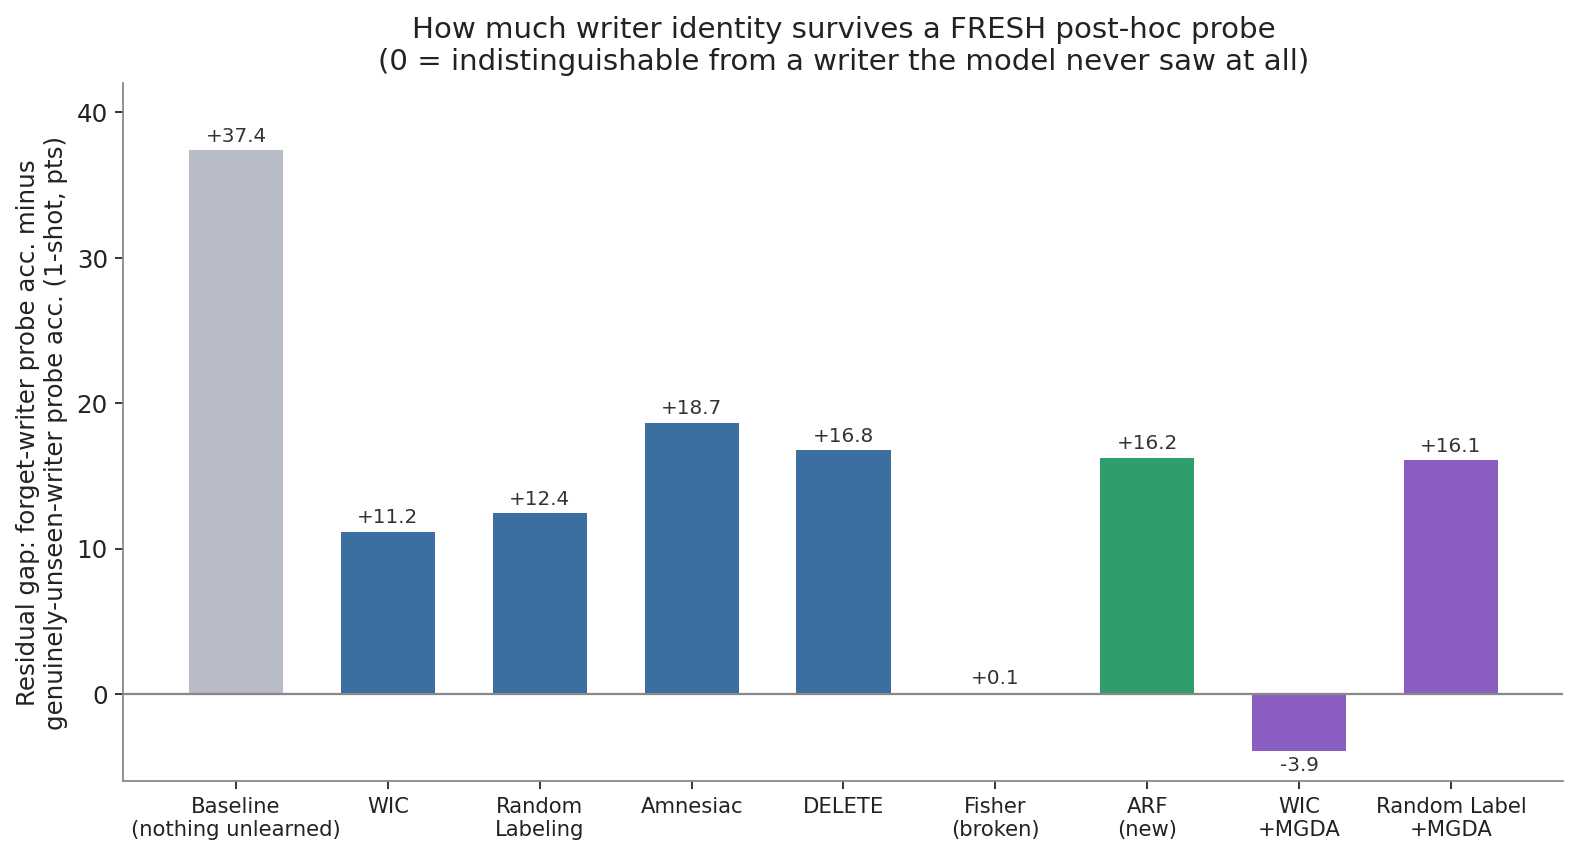
\includegraphics[width=\linewidth]{figs/fig_residual_gap_all_methods.png}
\caption{1-shot probe residual gap, all eight unlearning methods. ARF sits
squarely within the range of output-level methods, not below it.}
\label{fig:residual-gap}
\end{figure}

\begin{figure}[h]
\centering
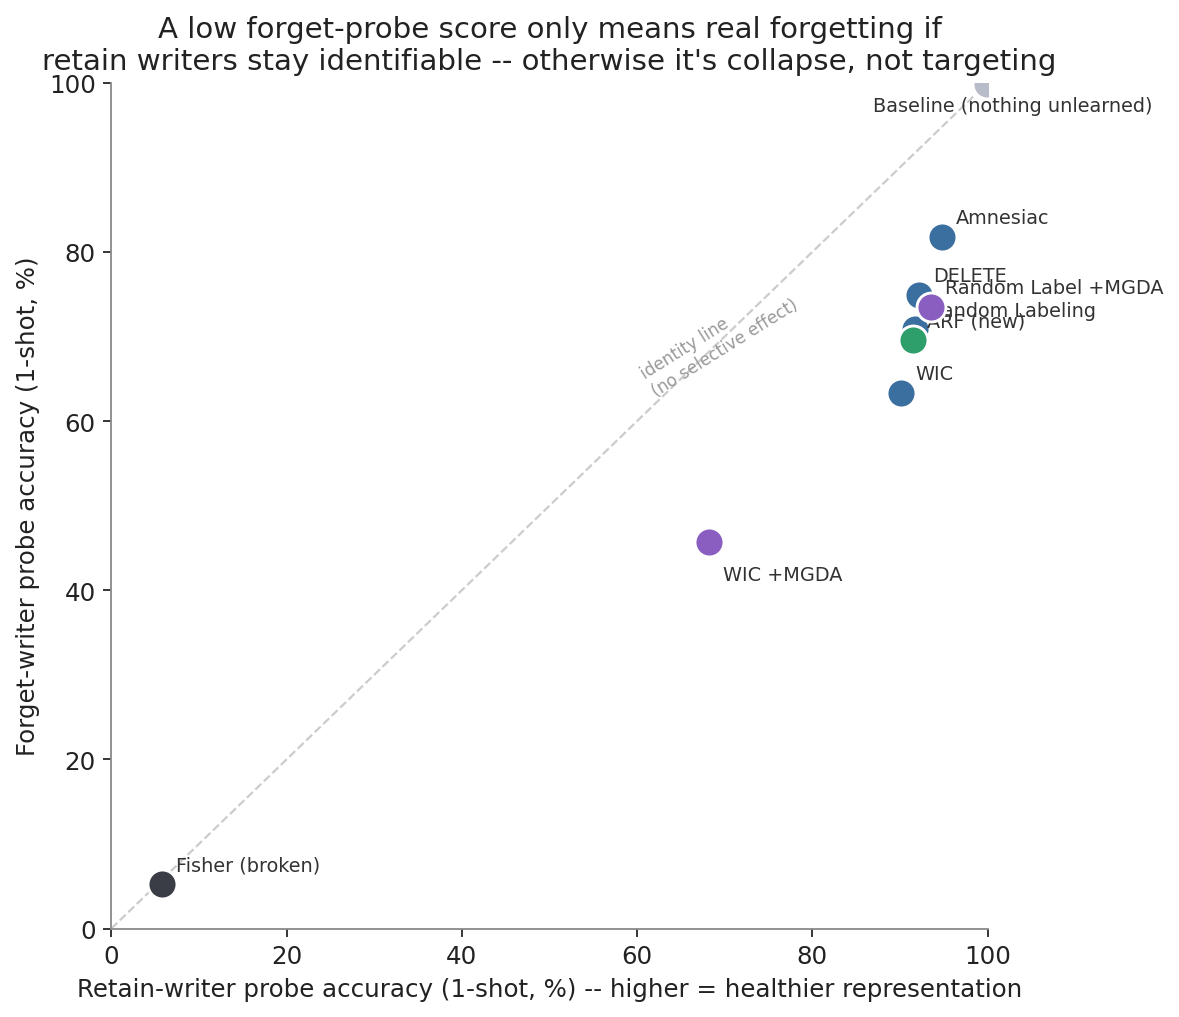
\includegraphics[width=\linewidth]{figs/fig_targeted_vs_collapse.png}
\caption{Forget-writer vs.\ retain-writer probe accuracy, one point per
method. WIC+MGDA sits off the pack toward the lower-left, indicating
general representational damage rather than selective forgetting.}
\label{fig:targeted-vs-collapse}
\end{figure}

\begin{figure}[h]
\centering
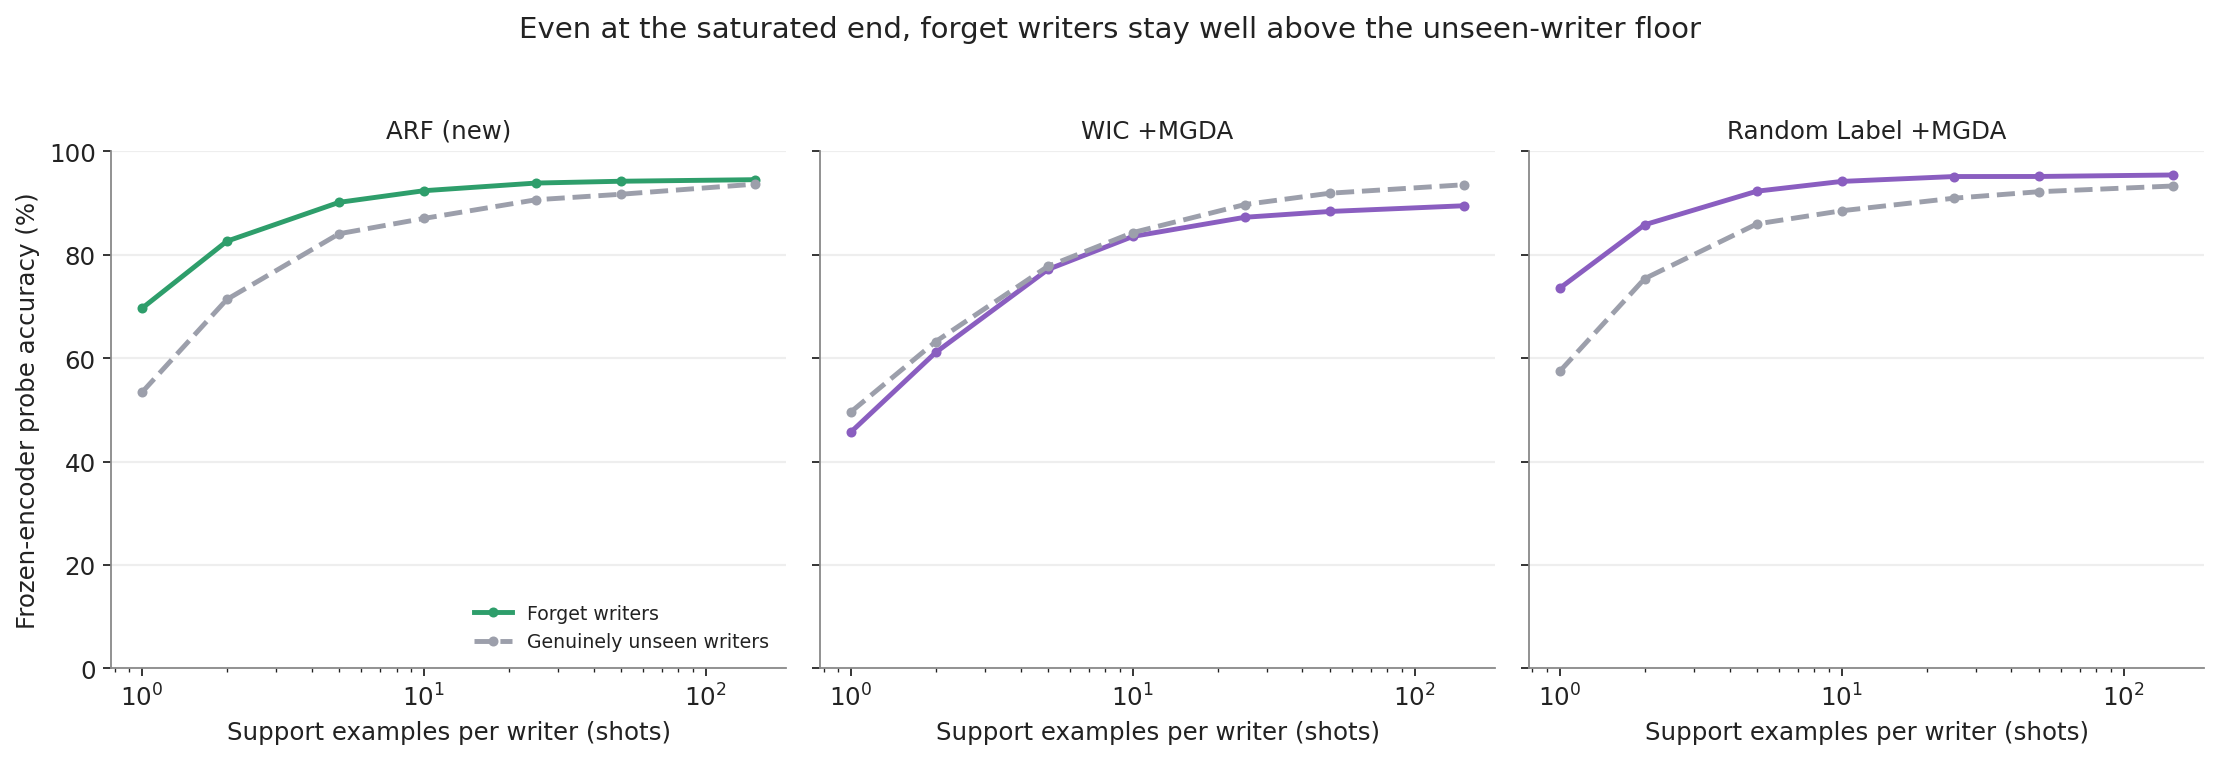
\includegraphics[width=\linewidth]{figs/fig_probe_curves_new_methods.png}
\caption{Frozen-encoder probe accuracy vs.\ shots per writer, forget vs.\
unseen writers, for the three new methods. The gap never closes, including
at saturation (150 shots).}
\label{fig:probe-curves}
\end{figure}

\begin{figure}[h]
\centering
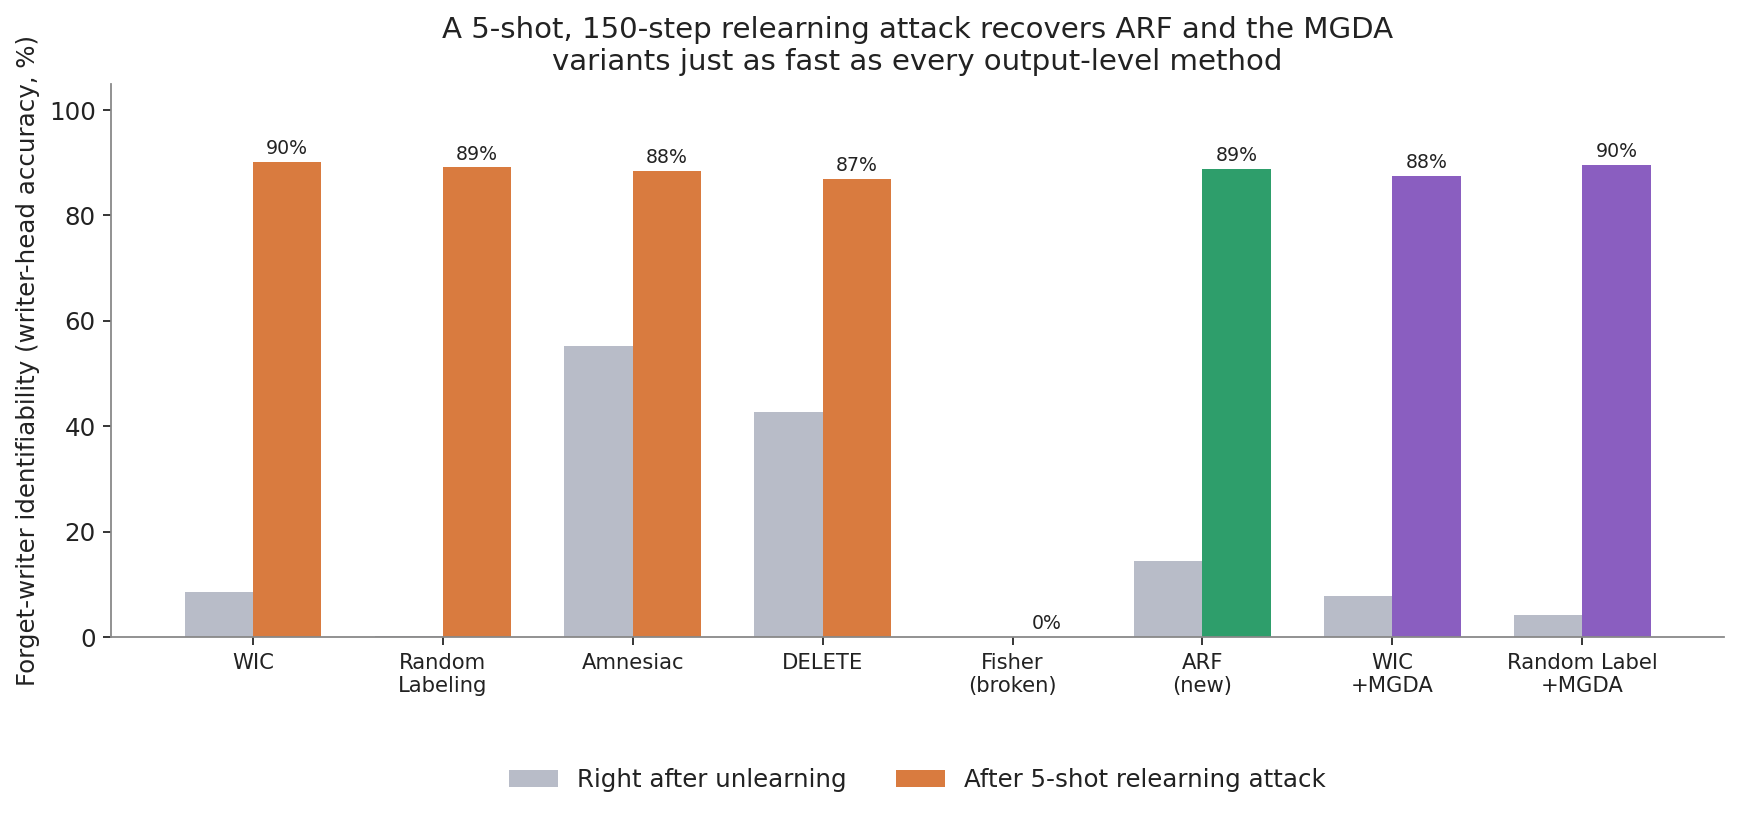
\includegraphics[width=\linewidth]{figs/fig_relearn_recovery_all_methods.png}
\caption{Relearning-attack recovery (5-shot, 150 steps), all eight
methods. ARF and both MGDA variants recover as fast as every output-level
method.}
\label{fig:relearn-recovery}
\end{figure}

\begin{figure}[h]
\centering
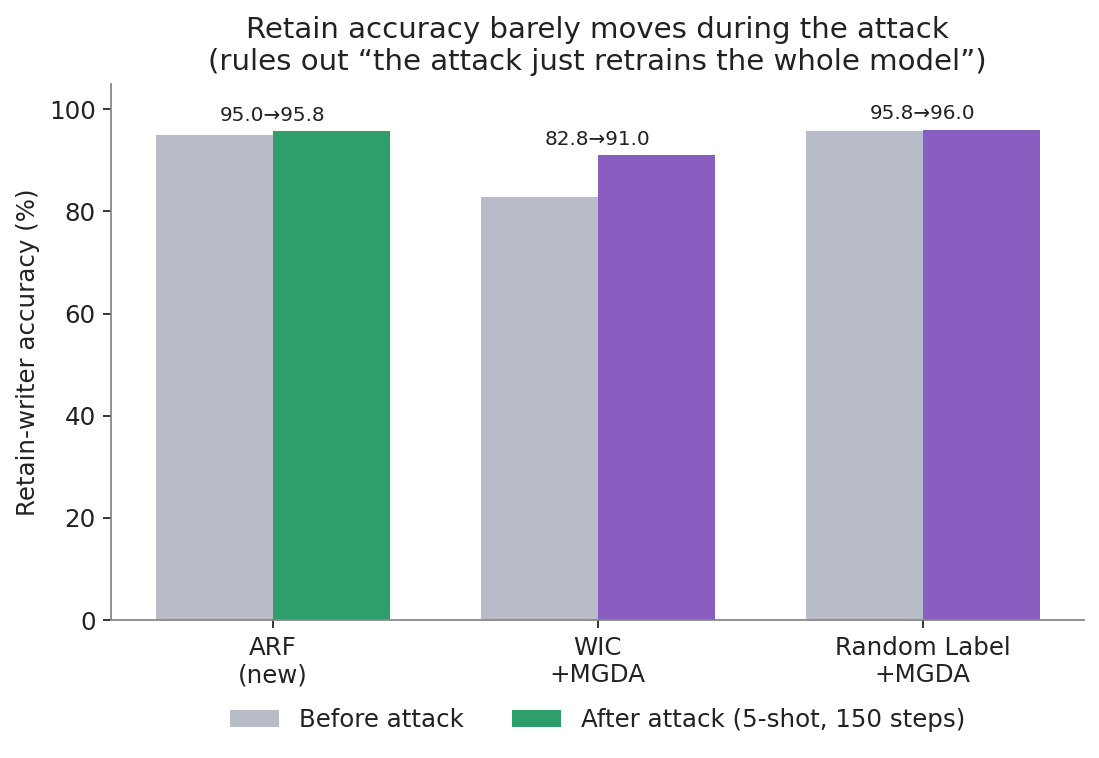
\includegraphics[width=\linewidth]{figs/fig_retain_stability_new_methods.png}
\caption{Retain-writer accuracy before/after the relearning attack, three
new methods.}
\label{fig:retain-stability}
\end{figure}

ARF's own training-time adversary is driven to 0\% accuracy during
training -- internally, the attack looks completely successful. Table
\ref{tab:probe} and Figure~\ref{fig:residual-gap} show that a
\emph{fresh}, independently-trained probe still recovers forget-writer
identity at 69.6\% 1-shot accuracy, a residual gap (+16.2~pt) \emph{larger}
than plain WIC's (+11.2~pt), and Figure~\ref{fig:relearn-recovery} shows a
relearning-attack recovery (88.9\% at 5-shot) indistinguishable from every
output-level method. Fooling one adversary, however sophisticated or
however often refreshed, does not establish that a \emph{different}
adversary cannot still succeed against the same representation.

We tested this directly with a five-arm ablation over the ARF adversary's
capacity (a deeper 3-layer probe at full hidden width instead of the
original 2-layer, halved-width one), ensemble size (3 concurrently-trained
probes the encoder must fool jointly), reset cadence (every 25 steps
instead of 100, and never), and loss weight (\texttt{LAMBDA\_ADV} and
\texttt{GRL\_LAMBDA} raised $3\times$), each otherwise identical to the
original ARF run (800 iterations, same Stage~I pruning, same retain
objective). The result complicates the single-configuration verdict above.
A deeper probe (\texttt{arf\_deepprobe}, residual gap $+8.5$~pt) and a
3-probe ensemble (\texttt{arf\_ensemble3}, $+11.0$~pt) both reach a
\emph{smaller} residual gap than every original output-level method,
including WIC's previous best of $+11.2$~pt -- and, critically, without the
collapse confound that invalidated WIC+MGDA's apparent win: 1-shot
retain-writer probe accuracy stays at 91.3\% and 91.6\% respectively,
close to the healthy range every other working method occupies, not the
68.2\% collapse floor. A faster reset cadence
(\texttt{arf\_reset25}, $+12.4$~pt, 91.4\% retain) shows the same pattern
more weakly; never resetting the probe (\texttt{arf\_noreset}, $+15.6$~pt,
89.9\% retain) is roughly indistinguishable from the original ARF
configuration. Scaling the loss weights $3\times$
(\texttt{arf\_strongadv}) looks worse by the residual-gap number alone
($+22.4$~pt) but this reading is confounded exactly the way WIC+MGDA's was:
1-shot retain-writer probe accuracy drops to 76.6\%, a clear partial
collapse rather than a cleaner failure to forget.

This means the answer to Experiment 6's motivating question is neither
``adversary capacity was the whole story'' nor ``the representation is
simply redundant, full stop.'' A stronger adversary -- specifically
deeper or ensembled, not simply more aggressively weighted -- recovers
less forget-writer information than the original single-configuration ARF
run, and less than any output-level method tested in this paper, while
leaving retain-writer information intact. The original ARF result
therefore understated what representation-level attacks can achieve; it
was, in part, an adversary-capacity ceiling rather than proof that the
representation cannot be attacked more effectively. It was not, however, a
capacity ceiling that naive loss-weight scaling removes -- that axis
degrades into the same general representational damage MGDA's aggressive
weighting produced. None of the five variants reaches a residual gap near
zero: even the best ($+8.5$~pt) leaves forget-writer identity clearly
above the unseen-writer floor, so the qualitative conclusion --
representation-level attacks alone do not achieve the kind of forgetting
their training-time success metrics suggest -- still holds. It holds by a
narrower margin than the original single-run comparison implied.

MGDA weighting is a mixed result, not a clean improvement on either
baseline it modifies. Random Labeling+MGDA is statistically
indistinguishable from fixed-weight Random Labeling on every metric.
WIC+MGDA's apparent win in Table~\ref{tab:probe} -- the only \emph{negative}
residual gap in this study -- does not survive Figure
\ref{fig:targeted-vs-collapse}: its retain-writer probe accuracy also
collapsed (68.2\% vs.\ 90\%+ for every other working method), and its
retain-set accuracy \emph{recovers} 8.25 points during the relearning
attack rather than holding steady (Table~\ref{tab:relearn},
Figure~\ref{fig:retain-stability}) -- the signature of general
representational damage, not a targeted effect.

\begin{table}[h]
\caption{Summary verdict, representation-level methods and the Experiment~6
ARF ablation suite. Residual gap is the 1-shot CLS-probe forget-minus-unseen
accuracy; retain is 1-shot retain-writer probe accuracy, the collapse check.}
\label{tab:verdict}
\begin{tabular*}{\tblwidth}{@{}LLLLL@{}}
\toprule
Method & Attacks & Residual gap & Retain & Verdict \\
\midrule
ARF & Representation & +16.2 pt & -- & No better than output-level \\
ARF+deep probe & Representation & +8.5 pt & 91.3\% & Better than any output-level arm \\
ARF+3-ensemble & Representation & +11.0 pt & 91.6\% & Better than any output-level arm \\
ARF+reset25 & Representation & +12.4 pt & 91.4\% & Modest improvement \\
ARF+no reset & Representation & +15.6 pt & 89.9\% & $\approx$ original ARF \\
ARF+3$\times$ weight & Representation & +22.4 pt & 76.6\% & Collapse, not forgetting \\
WIC+MGDA & Head (weighted) & $-3.9$ pt & 68.2\% & Collapse, not forgetting \\
RL+MGDA & Head (weighted) & +16.1 pt & -- & No change vs.\ fixed weights \\
\bottomrule
\end{tabular*}
\end{table}

\begin{figure}[h]
\centering
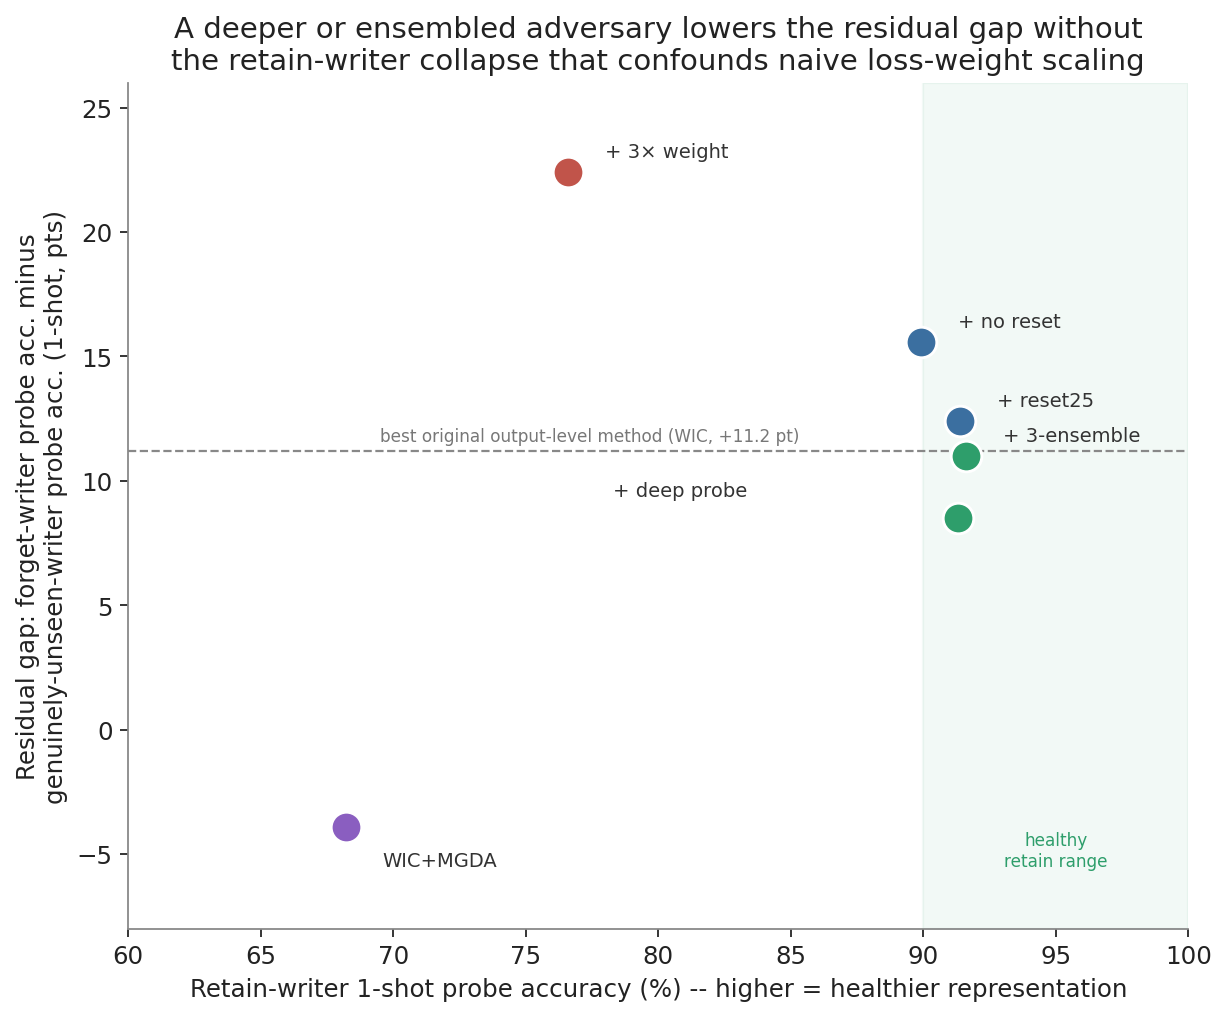
\includegraphics[width=\linewidth]{figs/fig_arf_capacity_ablation.png}
\caption{Residual gap vs.\ retain-writer probe accuracy, Experiment~6's
five-arm ARF capacity ablation plus WIC+MGDA. The deep-probe and
3-ensemble arms sit below the dashed best-output-level-method line
\emph{and} inside the healthy retain range (shaded); the $3\times$-weight
arm and WIC+MGDA reach a low residual gap only by also destroying
retain-writer information -- collapse, not forgetting.}
\label{fig:arf-capacity}
\end{figure}

A capacity/architecture control was attempted with a stronger encoder than
ResNet-18: ConvNeXt-Base, chosen specifically because it is designed to
match ViT-level performance using only convolutional operations, isolating
architecture family from the confound of ResNet-18's much smaller capacity
and weaker aggregate accuracy (Table~\ref{tab:encoder-ablation}). A
ConvNeXt-Base backbone was wrapped to mimic the ViT encoder's call
interface (a learned CLS token at position~0, projected to the same
768-dimensional space the pretrained TrOCR decoder's cross-attention
expects, with a 2D sinusoidal position encoding computed from the actual
feature-map size) and trained jointly with the writer head under the
identical protocol as every other arm.

\begin{table}[h]
\caption{ConvNeXt-Base architecture-control attempt, 8 epochs, writer-disjoint split.}
\label{tab:convnext}
\begin{tabular*}{\tblwidth}{@{}LLLL@{}}
\toprule
Eval.\ set & Word/Writer ACC (\%) & CER (\%) & WER (\%) \\
\midrule
Forget (writer-ID) & 0.00 & -- & -- \\
Retain (writer-ID) & 5.00 & -- & -- \\
Forget (recognition) & -- & 0.27 & 0.27 \\
Retain (recognition) & -- & 0.17 & 0.40 \\
Test (recognition) & -- & 7.58 & 17.33 \\
\bottomrule
\end{tabular*}
\end{table}

The recognition side of this result is a genuine, useful finding on its
own: ConvNeXt-Base's held-out test CER (7.58\%) sits close to the TrOCR ViT
oracle's (7.74\%, Table~\ref{tab:probe}'s companion result), confirming
that a pure-convolutional architecture \emph{can} match Transformer-level
handwriting recognition when given comparable capacity -- exactly the
premise ConvNeXt was designed around, and the reason it was chosen over a
plain ResNet. Section~\ref{sec:apples-to-apples} tightens this comparison
considerably: under the standard (non-writer-disjoint) split and beam-4
decoding this paper's headline number itself uses -- rather than the
writer-disjoint, greedy-decoded protocol this section requires -- ConvNeXt
lands within half a point of ViT on word accuracy, the strongest evidence
in this paper that the recognition gap between the two architectures is
close to a genuine tie.

The writer-identification side did not work: retain-writer accuracy
reached only 5.00\% (chance $\approx 1.35\%$ over 74 classes) and
forget-writer accuracy was 0.00\%, against $\sim$100\%/100\% for the TrOCR
ViT baseline under the identical joint-training recipe
(Table~\ref{tab:unlearn-all}). The gate check
(Section~\ref{sec:unlearn-pipeline}) accordingly failed, and Stage~I/II
pruning and unlearning were not run against this checkpoint: a model whose
writer head has not learned to discriminate writers in the first place
gives no meaningful signal about \emph{unlearning} resistance, since there
is nothing to forget. We report this as a limitation rather than force a
Stage~I/II run on an uninformative baseline (Section~\ref{sec:limitations}).
Two explanations were equally consistent with the numbers above: (i) a
genuine architectural dissociation, where ConvNeXt's locally-built-up
convolutional features support content recognition well but do not
naturally summarize into a single token carrying a global, holistic style
signature the way a Transformer's attention-pooled CLS representation
does; or (ii) an artifact of this specific adapter, whose CLS token has no
pretraining signal and might simply need more aggressive tuning to
specialize for identity alongside a recognition objective that converges
quickly on this architecture.

We tested explanation (ii) directly rather than leaving it open. A second
run gave the CLS token, its projection, and the writer head their own
optimizer parameter group at $20\times$ the base learning rate (instead of
sharing the same rate as the rest of an already ImageNet-pretrained
backbone), and raised \texttt{WRITER\_W} $5\times$ (2.0 to 10.0) to force
substantially more gradient signal into the writer objective relative to
recognition. If explanation (ii) were correct, this should have moved
writer accuracy measurably even if it did not close the gap entirely. It
did not move at all: validation writer accuracy was 4.00\% at every one of
8 epochs, unchanged to two decimal places, while recognition CER improved
normally over the same schedule (22.2\% $\to$ 3.8\%) -- confirming the
optimizer change was active and the two objectives were not simply both
stalled. Final forget/retain writer accuracy (0.00\%/5.00\%) was
statistically indistinguishable from the untuned run. A $20\times$
learning-rate increase and $5\times$ loss-reweighting on the exact
parameters responsible for writer identification producing zero
measurable change is difficult to reconcile with explanation (ii): an
under-trained token that was merely slow to specialize should show
\emph{some} response to an intervention this aggressive. This shifts the
weight of evidence toward explanation (i) -- a genuine architectural
property, not an artifact of this study's specific adapter -- though a
single dataset and a single tuning attempt cannot rule out (ii) entirely;
Section~\ref{sec:limitations} treats this as the next-lowest-hanging
open question, and a second dataset (not necessarily a different
language, since the recognition side already generalizes across script
complexity) would be the natural way to close it.

We then closed that open question directly with a second, independent
Bangla dataset: BanglaWriting~\citep{mridha2021banglawriting}, 260
writers and 21,234 words of single-page handwriting with word-level
bounding-box annotations, collected under a completely different
acquisition pipeline than BnHTRD and sharing no writers with it. Using
the identical joint recognition-plus-writer-identification recipe (the
already-tuned $20\times$/$10\times$ ConvNeXt configuration, applied from
the start rather than re-derived) and a fresh character-level decoder
vocabulary sized to this dataset, both encoders were trained for 6
epochs on a sample-level (not writer-disjoint) split, so that every
writer appears in both train and validation and a low score cannot be
explained by a writer the model never saw. The result reproduces the
BnHTRD dissociation almost exactly: the TrOCR ViT encoder reached
68.30\% validation writer-identification accuracy (chance $\approx
0.38\%$ over 260 classes), while ConvNeXt-Base reached 0.75\% --
statistically indistinguishable from chance -- despite both encoders'
recognition loss falling on comparable schedules (ConvNeXt: 1.64 $\to$
0.03 over the same 6 epochs, confirming the encoder and decoder were
training normally throughout). With this second, independently
collected Bangla dataset now agreeing with BnHTRD, and the earlier
tuning attempt already having ruled out an under-trained-adapter
explanation on BnHTRD itself, the evidence for explanation (i) -- that
ConvNeXt's convolutional features do not naturally pool into a
holistic, writer-discriminative summary the way a Transformer's
attention-pooled CLS token does, independent of the specific dataset --
is now substantially stronger than a single-dataset result could
support.

\paragraph{A brief cross-script side note.} This paper's focus is Bangla,
and the two results above are its evidence. As a lightweight robustness
check on a single additional run -- not a central claim, and not powered
or repeated the way the Bangla comparisons above are -- the same recipe
was also tried once on Felix92/ibm-handwriting-campaign-word, an English
(Latin-script) dataset of 300 writers, to see whether the dissociation
found on Bangla is specific to that script. The result is a smaller
version of the same gap, not an identical one. ViT again dominated
(88.61\% vs.\ chance $\approx 0.33\%$), and the \emph{relative}
ViT/ConvNeXt gap stayed at least an order of magnitude, consistent with
both Bangla runs (BnHTRD $\sim$20$\times$; BanglaWriting $\sim$91$\times$;
English $\sim$30$\times$) -- but ConvNeXt's \emph{absolute} accuracy here
(2.91\%, $\sim 8.7\times$ chance) was a small, real, non-chance signal,
unlike either Bangla dataset ($\sim2$--$4\times$ chance, statistically
indistinguishable from noise). Figure~\ref{fig:convnext-3} summarizes all
three datasets on one log-scaled axis.

One plausible, entirely unverified explanation is script structure
itself. Bangla's consonant conjuncts compose two or more base graphemes
into a single visually merged unit (Section~\ref{sec:tokenizers}), so a
writer's personal style plausibly manifests partly in \emph{how} those
units get assembled stroke-to-stroke -- a compositional, longer-range
property that a global-attention \texttt{[CLS]} token is architecturally
well-suited to summarize, and that a convolutional layer's local
receptive field is not, at least not without enough stacked depth to
span a multi-grapheme unit. Latin letterforms do not compose this way:
each letter in the English dataset is written as a single, non-conjunct
unit, so writer-specific stroke variation may sit more within one
letter's span -- closer to where a convolutional encoder's local
inductive bias is actually strong. This would predict exactly the
pattern observed (a narrowed but not closed gap on English) without
requiring the Bangla result to be wrong; it is a hypothesis this study
did not test directly, not a demonstrated mechanism.

\openq{The English run isolates script only if it is otherwise comparable
to the two Bangla runs, and it is not: it also differs in dataset,
writer population, and (unavoidably) language, all confounded with script
in this single comparison. Each of the three datasets was also run only
once, so it is not yet possible to separate a genuine script effect from
ordinary run-to-run variance on a signal this close to the noise floor.
A sharper test would hold conjunct-forming structure roughly comparable
while changing script (e.g.\ Bangla vs.\ Devanagari, both of which form
similar consonant conjuncts, rather than Bangla vs.\ Latin, which differs
in conjunct structure \emph{and} script \emph{and} dataset simultaneously),
or would repeat each of the three existing runs to put an error bar on
ConvNeXt's already-tiny writer-ID accuracy before reading anything into
whether it sits at 2--4$\times$ or 8--9$\times$ chance.}

\begin{figure}[h]
\centering
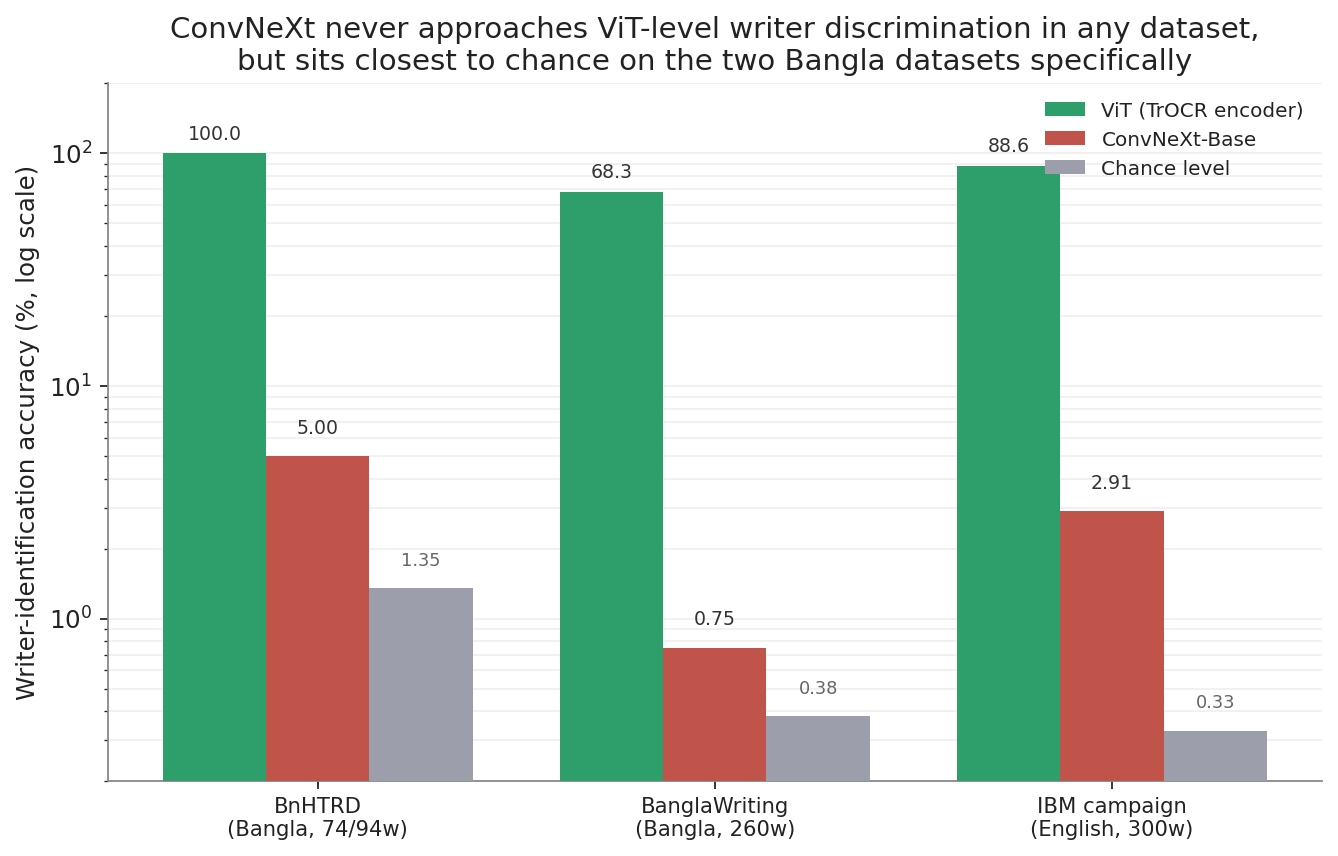
\includegraphics[width=\linewidth]{figs/fig_convnext_three_datasets.png}
\caption{ConvNeXt-Base vs.\ ViT writer-identification accuracy, all three
datasets, log scale. The relative gap (ViT over ConvNeXt) is at least an
order of magnitude everywhere; ConvNeXt's absolute distance from chance
is what varies -- indistinguishable from chance on both Bangla datasets,
a small but real signal on the English one.}
\label{fig:convnext-3}
\end{figure}

%% ====================================================================
\section{Discussion}
\label{sec:discussion}
%% ====================================================================

Two results, otherwise unrelated, trace to the same property. TrOCR's ViT
encoder produces a rich, general-purpose visual representation of
handwriting style -- 197 patch embeddings a cross-attention decoder can
selectively attend over, pretrained on large-scale handwritten-OCR corpora
-- and that representational richness is \emph{why} it beats ResNet-18 by
8.33 points Word Accuracy (Table~\ref{tab:encoder-ablation}). The same
richness is \emph{why} a writer's identity survives all five Kang et
al.\ unlearning objectives, and the purpose-built ARF attack, at the
representation level (Sections~\ref{sec:unlearn-results}--\ref{sec:arf-results}):
a representation expressive enough to generalize across 74 retain writers
is expressive enough to keep a forgotten writer's style linearly separable
long after the classification head sitting on top of it has been driven to
chance.

There is a second, methodological throughline. Corpus-level CER/WER made
grapheme tokenization's advantage look like a modest aggregate improvement;
only a paired, sample-level significance test (Section~\ref{sec:sample-sig})
revealed it is a large, mechanism-explicable effect concentrated in a
specific word class. Symmetrically, output-level unlearning metrics
(writer-head accuracy, a static MIA) made forgetting look complete; only
representation-level probing and an adversarial relearning attack revealed
it was not. In both halves of this paper, \textbf{aggregate, output-level
evaluation was not sufficient on its own} -- the real effect, in one
direction or the other, only appeared one level below the standard metric.

Two threads from the Results section are worth flagging explicitly here
rather than folding silently into the narrative above. First, the
apparent character/BPE crossover at the longest words
(Section~\ref{sec:complexity}) does not survive formal testing
($p=0.29$): it is better read as a hypothesis for why an underpowered
tail bucket's point estimate moved than as an established effect, and a
properly powered follow-up (deliberately oversampling long words) would
be needed before treating autoregressive error accumulation as a
confirmed mechanism rather than a plausible story fitted to noise.

\openq{Second, Section~\ref{sec:arf-results}'s five-arm ARF ablation shows
a deeper or ensembled adversary lowers the residual gap without the
retain-writer collapse a naive loss-weight increase causes, but does not
resolve \emph{why} it stops where it does: whether a still-deeper or
larger-ensemble adversary would keep closing the gap toward zero, or
asymptote above it the way the near-identical performance of
\texttt{arf\_noreset} to the original configuration might suggest. A
wider capacity grid run to convergence, with retain accuracy tracked
throughout rather than only at start and end, would be needed to
distinguish a capacity ceiling that keeps receding under a stronger
adversary from one that this study's five configurations have already
reached.}

Third, why does PATHOK's representation resist \citet{wang2026rfuss}'s
own attack strategy here, when RFU-SS achieves near-complete backdoor
removal under 0.2\% accuracy cost on its own benchmark? Two differences
are each independently sufficient to explain the gap without either
study's own numbers being unreliable on their own terms. Architecturally,
RFU-SS is evaluated on a small classifier trained from scratch under an
explicit Variational Information Bottleneck objective, whose stochastic
bottleneck is specifically designed to make later erasure of targeted
information tractable; PATHOK's ViT encoder is richly pretrained on
large-scale handwritten-OCR data with no such bottleneck, and
retrofitting one (Section~\ref{sec:arf-mgda}) was out of scope for this
study. Task-wise, RFU-SS erases an artificially injected, spatially
localized backdoor trigger -- a signal the model was never asked to
generalize from, occupying a small, learnable region of input space --
while this paper erases a writer's natural, holistic handwriting style, a
signal the recognition objective specifically rewards the encoder for
representing well across every example from that writer. An artificial,
localized signal being easier to excise than a natural, distributed one
is the more parsimonious reading of the gap between the two studies'
results than assuming either result does not hold on its own benchmark.

%% ====================================================================
\section{Limitations}
\label{sec:limitations}
%% ====================================================================

\begin{itemize}
\item The sample-level divergence analysis (Section~\ref{sec:sample-sig})
  is single-dataset (BnHTRD); the triple-divergence subgroup is small
  ($n=104$), so the per-conjunct rates in Figure~\ref{fig:top-conjuncts}
  are illustrative rather than independently significant.
\item Stage~I pruning's forget/retain activation gap was previously shown
  statistically indistinguishable from a null-distribution control
  (permutation $p=0.286$) and was not re-validated in this pass; the
  pruning step's contribution to Table~\ref{tab:unlearn-all} should not be
  read as validated targeting of forget-specific structure.
\item The relearning attack's recovery target is the original baseline's
  forget-writer accuracy rather than a retrain-from-scratch oracle; an
  oracle checkpoint was not available among this study's Kaggle kernel
  inputs for the ARF/MGDA arms specifically (the same limitation applies
  to the original five methods).
\item ARF ports the \emph{strategy} of \citet{wang2026rfuss} (attack the
  representation, not the head) via gradient reversal, not their literal
  Variational Information Bottleneck architecture or mutual-information
  loss. A more faithful reproduction -- retrofitting a stochastic VIB
  bottleneck into the PATHOK encoder -- was out of scope for this study and
  may behave differently, though Section~\ref{sec:discussion} argues the
  architecture and task gap would likely still apply.
\item The architecture/capacity control proposed to more directly test the
  throughline of Section~\ref{sec:discussion} (does a non-Transformer
  encoder resist unlearning less?) was attempted with ConvNeXt-Base rather
  than ResNet-18, specifically to hold recognition capacity roughly
  constant while varying architecture family
  (Section~\ref{sec:arf-results}). It did not reach the unlearning stage:
  the writer-identification head failed to learn (5.00\% retain accuracy
  against $\sim$100\% for the TrOCR ViT arm) despite recognition CER/WER
  closely matching the ViT arm, so Stage~I/II pruning and unlearning were
  not run against this checkpoint. A follow-up tuning attempt ($20\times$
  learning rate on the fresh CLS-token/projection/writer-head parameters,
  $5\times$ higher \texttt{WRITER\_W}) produced no measurable change
  across 8 epochs, weakening the adapter-artifact explanation but not
  eliminating it outright -- a single tuning attempt on a single dataset is
  not conclusive. A second, independently collected Bangla dataset
  (BanglaWriting~\citep{mridha2021banglawriting}, 260 writers, no shared
  writers or acquisition pipeline with BnHTRD) was run as the natural next
  step instead of further same-dataset tuning, and reproduced the
  dissociation closely: 68.30\% ViT vs.\ 0.75\% ConvNeXt validation
  writer-identification accuracy (chance $\approx 0.38\%$), with both
  encoders' recognition loss falling normally throughout
  (Section~\ref{sec:arf-results}). This paper's claims rest on that
  Bangla-only evidence; a single, unrepeated side-note run on an English
  dataset (Felix92/ibm-handwriting-campaign-word, 300 writers) is reported
  in Section~\ref{sec:arf-results} \emph{only} as a preliminary check of
  whether the effect is Bangla-specific, not as a validated cross-script
  result -- it found the same order-of-magnitude relative gap but a small
  non-chance absolute ConvNeXt signal unlike either Bangla run, one
  plausible (unverified) reading of which is that Bangla's consonant
  conjuncts specifically call on the kind of compositional, longer-range
  summarization a Transformer's attention does and a convolution's local
  receptive field does not. Confirming this would need a same-script,
  cross-language comparison (e.g.\ against Devanagari, not Latin) and
  repeated runs per dataset, neither of which this study has. This
  still leaves the throughline's architecture-family claim resting on
  the correlational ResNet-18 comparison
  (Table~\ref{tab:encoder-ablation}) rather than a matched-capacity
  causal Stage~I/II unlearning run, since ConvNeXt never reached that
  stage on any of the three datasets.
\item Table~\ref{tab:gradet-compare}'s comparison against GraDeT-HTR uses
  each study's own reported numbers rather than a re-run under identical
  splits and preprocessing, and should be read as contextual rather than
  strictly controlled.
\end{itemize}

\todo{Add any additional limitations identified during expatiation.}

%% ====================================================================
\section{Ethical Considerations}
\label{sec:ethics}
%% ====================================================================

This study's own results show that output-level unlearning success metrics
-- writer-head accuracy, a static membership-inference gate -- are not
trustworthy evidence that a writer's biometric handwriting signature has
been removed from a trained model. Any deployment that promises
writer-level data deletion under a right-to-erasure request built on this
class of model therefore requires representation-level auditing (a
frozen-encoder probe and, ideally, an adversarial relearning attack), not
head-accuracy checks alone. Reporting Fisher Forgetting's outright failure
and the relearning attack's success against every other method, without
softening either result, is itself the ethical position of an audit study
of this kind.

\textbf{Societal.} A working Bangla HTR system carries a genuine societal
upside -- document digitization, administrative and archival backlog
reduction, and assistive technology for a script with comparatively
little existing tooling relative to its speaker population
(Section~\ref{sec:related-ocr}) -- and this study's contribution to that
system (grapheme tokenization's accuracy gain) does not itself raise new
societal risk beyond what any improved HTR system carries. The privacy
half of this paper exists specifically because that same accuracy gain
has a cost: the richer the representation, the more of a writer's
identity it appears to retain (Section~\ref{sec:discussion}), so
recognition improvements of the kind reported in
Section~\ref{sec:agg-results} should not be pursued without also
budgeting for the unlearning-auditing burden this paper documents.

\textbf{Health and safety.} Not applicable to this study: PATHOK is an
offline text-recognition system with no real-time, safety-, or
health-critical deployment context evaluated here.

\textbf{Legal and cultural.} This study treats handwriting as a
biometric identifier subject to a right-to-erasure-style expectation
(Section~\ref{sec:introduction}) without taking a position on any
specific jurisdiction's data-protection statute; readers deploying a
system of this kind should consult the actual data-protection and
consent-withdrawal law applicable to their jurisdiction and data source,
since this paper's own claim is narrower and empirical -- that
output-level unlearning metrics are not sufficient evidence of erasure --
rather than legal. BnHTRD and BanglaWriting are both publicly released
research datasets with their own stated consent and usage terms; this
study performs no new data collection from human subjects and did not
require separate institutional review beyond compliance with those
datasets' existing release terms.

\textbf{Environment and sustainability.} Every experiment in this paper
was run on single-GPU cloud instances (Section~\ref{sec:limitations}
documents the specific compute-availability constraints this imposed),
and no experiment here required large-scale distributed training; the
dominant compute cost is the nine-arm unlearning audit and its associated
relearning-attack sweep (Table~\ref{tab:unlearn-all}), repeated across
several encoder and tokenizer configurations. \todo{Report an aggregate
GPU-hour figure and, if feasible, an estimated carbon-equivalent figure
for the full experimental campaign before submission, per the target
venue's environmental-impact reporting expectations if any.}

%% ====================================================================
\section{Conclusion}
\label{sec:conclusion}
%% ====================================================================

This paper reproduces and extends two separate lines of prior work on a
single Bangla HTR system. On recognition, TrOCR with grapheme tokenization
reaches 92.21\% word accuracy and 2.52\% CER, and a sample-level,
paired-significance analysis shows the tokenizer effect is real,
statistically overwhelming, and concentrated specifically in
consonant-conjunct words -- going beyond the aggregate rankings reported by
prior Bangla HTR tokenizer studies. On privacy, five machine-unlearning
methods and two representation-level methods built for this study all
leave a Bangla handwriting model's memory of specific writers
recoverable, under both a frozen-encoder probe and a retain-replay-controlled
relearning attack, despite passing the output-level metrics the original
unlearning literature relies on. Both findings trace to the same property:
the rich, general-purpose visual representation that gives TrOCR its
recognition advantage over a convolutional baseline is exactly what
resists both script-agnostic tokenization and targeted removal --
and in both cases, aggregate output-level metrics were not sufficient
evidence on their own. A direct architecture-family check, run in place
of the originally proposed ResNet-18 forgetting-resistance control, adds a
third strand of evidence for this reading: replacing the ViT encoder with
a capacity-matched convolutional one (ConvNeXt-Base) preserves recognition
accuracy but not the writer-head's ability to learn identity in the first
place, confirmed on two independent Bangla datasets and unmoved by an
order-of-magnitude tuning intervention -- suggesting the representational
property this paper studies is not simply a function of model scale.

Several threads remain open, and this paper reports them as such rather
than rounding them off. On the recognition side,
Section~\ref{sec:complexity}'s vocabulary-size sweep leaves unresolved
whether grapheme tokenization's advantage reflects genuine
linguistic-unit alignment or simply a smaller, more stable vocabulary
(Section~\ref{sec:agg-results}). On the privacy side, the Experiment~6
ARF ablation (Section~\ref{sec:arf-results}) narrows but does not close
the gap to genuine forgetting, and whether a still-stronger adversary
would keep closing it or has already reached a ceiling is not resolved by
this study's five-point grid. On the architecture-family result, a single
side-note run on an English dataset (Section~\ref{sec:arf-results})
complicates the clean Bangla-only picture without a controlled
same-conjunct-structure comparison to explain why; and the causal version
of the architecture claim -- a matched-capacity, non-pretrained encoder
control taken all the way through Stage~I/II unlearning, which ConvNeXt's
writer-identification failure prevented in this study -- remains the most
direct missing piece connecting Table~\ref{tab:encoder-ablation}'s
correlational encoder comparison to Section~\ref{sec:discussion}'s
representational-richness explanation.

%% ====================================================================
\appendix
\section{Additional Qualitative Examples}
\label{sec:appendix}

\todo{Space reserved for additional qualitative material not yet built:
(i) a failure-case grid mirroring Figures~\ref{fig:qual-grid-bpe}/\ref{fig:qual-grid-triple}
but for words where \emph{grapheme} tokenization itself fails (currently
only grapheme-wins are shown; a reader should also be able to see what
the remaining $\sim$8\% of grapheme errors look like); (ii) a per-writer
breakdown of Table~\ref{tab:unlearn-all}'s forget-writer accuracy (are the
20 forget writers unlearned uniformly, or does resistance concentrate in
a few high-sample-count writers?); (iii) qualitative examples from the
BanglaWriting and English cross-dataset runs
(Section~\ref{sec:arf-results}) analogous to
Figures~\ref{fig:qual-grid-bpe}--\ref{fig:qual-grid-triple}, to make the
ConvNeXt/ViT writer-ID dissociation visually inspectable rather than
purely numeric. None of these three requires new experiments -- all three
datasets and checkpoints already exist -- only additional analysis and
plotting passes over data already collected.}

\printcredits

\bibliographystyle{cas-model2-names}
\bibliography{refs}

\end{document}
